\documentclass{sty/eiiatfg}

\usepackage[nomain,acronym]{glossaries}
\makeglossaries

% Hay muchos paquetes para LaTeX que facilitan centenares de trabajos
% engorrosos. Busca en Internet si no sabes hacer algo con LaTeX. El
% repositorio oficial está en https://ctan.org/

% Algunos paquetes especialmente útiles ya están incluídos en el estilo
% del TFG (consulta sty/eiiatfg.cls para más detalles).

% Cambia los datos de tu TFG en este archivo

\title{Sistemas de control en modelos de comportamiento colectivos}
\author{Pablo Mateos Corrales}

% IE = Ingeniería Eléctrica
% IEIA = Ingeniería Electrónica Industrial y Automática
% IA = Ingeniería Aeroespacial
\grado{IEIA}

% Tu número de expediente puedes consultarlo en secretaría virtual
\expediente{225172}

% En caso de múltiples directores separa los nombres con \\
% Si solo hay un tutor no pongas \\
\tutor{%
    Jesús Rosado Linares}


% A partir de aquí se trata de datos opcionales. Si algún dato no quieres que figure borra la línea o coméntala poniendo el signo % al principio

% Es muy conveniente proporcionar un medio de contacto con el autor.  El correo electrónico es probablemente el menos invasivo. No uses correos con nicknames extraños, es un documento profesional. En caso de duda usa el correo de la Universidad, pero recuerda que dejará de ser válido unas semanas después de que dejes de ser alumno.
\email{pablo.mateos@alu.uclm.es}

% No uses tu teléfono personal, será accesible para cualquier usuario de la biblioteca
\phone{925 268 800 x.3729}

% Una página web para el proyecto puede ser un requisito necesario en caso de que sea trabajo parcialmente financiado con un proyecto de I+D. Consulta a tu tutor
\homepage{https://github.com/pmateosc/eii-tfg}

% Tener un repositorio GIT (http://github.com) permite llevar un control de versiones. Tu tutor puede considerarlo esencial, habla con él
\gitrepo{https://github.com/pmateosc/TFG-22-B-225172}

% Pon una dirección si puede ser interesante para recibir correspondencia relacionada. No pongas tu dirección personal
\address{UCLM --- Escuela de Ingeniería Industrial y Aeroespacial\\
    Campus Universitario de la Real Fábrica de Armas}
\poblacion{Toledo}
\cpostal{45071}

% Definición de acrónimos:
% \newacronym{id}{corto}{largo}

% Uso de acrónimos
% \acrshort{id} nombre corto
% \acrlong{id}  nombre largo
% \acrfull{id}  nombre largo (nombre corto)

\newacronym{SI}{SI}{Swarm Intelligence}
\newacronym{CS}{CS}{Cucker Smale}
\newacronym{CCR}{CCR}{Cañizo Carrillo y Rosado}



% La bibliografía la puedes descomponer en varios archivos .bib
% Los archivos .bib se pueden escribir a mano con ayuda de un editor online
% (e.g. http://truben.no/latex/bibtex) o generar con Mendeley u otro
% gestor de bibliografía. Solo se incluyen las referencias que son citadas
% en el texto.
\addbibresource{bib/main.bib}

\begin{document}

% Puedes cambiar la licencia de este documento con la orden license.  Por defecto se asume Creative Commons Attribution 4.0 (ver https://creativecommons.org/licenses/by/4.0/).  
% Por ejemplo, para restringir su uso, copia y distribución:
%\license{Todos los derechos reservados.}

% Si usas muchos símbolos conviene que describas lo que significan en un archivo
% aparte (en este caso simbolos.tex).  Si no es el caso puedes comentar esta línea
%\listofsymbols{simbolos.tex}


\portada

% Edita los
\begin{agradecimientos}
En primer lugar, quiero agradecer a mi tutor, Jesús Rosado, su dedicación y su entusiasmo por orientarme en un área de las Matemáticas tan desconocido como complicado para mí. También quiero agradecer la labor que ejercen los profesores de la Escuela, que tanto me han enseñado, en especial a Fernando Castillo, José Luis Polo e Ismael Payo, que personalmente me han enseñado a sentir pasión por la Ingeniería y a perseguir la excelencia.

También quiero agradecer a mi familia, el esfuerzo que han hecho siempre para que yo pudiera realizar y terminar la carrera y el apoyo que han supuesto en los momentos más complicados. Gracias papá por inculcarme el valor del conocimiento y enseñarme a estudiar. Gracias mamá por tu cariño y delicadeza han curado muchas caídas en la carrera. María, gracias por apoyarme y animarme a terminar el TFG con tu empatía y comprensión.

Acuña, Noemí, Ismael, Miguel Ángel, gracias por aparecer en mi vida universitaria y convertiros en mi familia para lo bueno y lo malo.
\end{agradecimientos}	   
\begin{dedicatoria}
A mi abuelo Antonio.
\end{dedicatoria}
\begin{resumen}

El objeto principal de este Trabajo Fin de Grado es conocer en profundidad modelos de comportamiento colectivo, más concretamente, el modelo de Cucker Smale y dos modelos adicionales que añaden un control, el modelo propuesto por Cañizo y col. \cite{canizo2010collective} y el propuesto por Trèlat y col. \cite{caponigro2015sparse}. Cucker Smale propone un modelo que pretende describir el comportamiento colectivo en bandadas de pájaros, aportando un sistema de ecuaciones que responde y es capaz de simular ese comportamiento en función, principalmente, del llamado parámetro de convergencia, $\beta$. Los autores que intervienen en el modelo de Cañizo, proponen un modelo basado en el de Cucker Smale al cual añaden la influencia que ejercen unos individuos sobre otros en función del promedio de la velocidad relativa del grupo y Trèlat y col. centran sus estudios en una premisa muy clara que es reducir el gasto energético que conlleva controlar el grupo hasta conseguir el consenso, centrándose así en generar un impulso mayor sobre el individuo más desviado.

Todos los modelos anteriores se han implementado en Matlab de manera que fuera posible obtener datos que permitan comparar el comportamiento del grupo al regirse por unas reglas u otras. Tras estas simulaciones se ha podido mostrar por una parte que el modelo de Cañizo es el más rápido en llegar a un estado de consenso bajo condiciones que ayuden conseguirlo y el de Trèlat que impulsa sólo a un individuo consigue llegar al consenso con menor gasto energético, en un tiempo finito ligeramente mayor, y por otra parte que bajo condiciones que compliquen el consenso, es Trélat quien tiene más facilidades para conseguirlo.

\end{resumen}

\begin{abstract}
The main purpose of this undergraduate thesis is to know in depth the collective behavior models, specifically, the Cucker Smale model and two additional control models, the model proposed by Cañizo et al. \cite{canizo2010collective} and the one proposed by Trèlat et al. \cite{caponigro2015sparse}. Cucker Smale propose a model to describe the behavior of a flock of birds, providing a system of equations that is capable of simulating that behavior based mainly on the so-called convergence parameter, $ \beta $. The authors involved in the Cañizo model propose a model based on the Cucker Smale one to which they add the influence exerted by some individuals on others based on the average relative speed of the group, and Trèlat et al. focus their studies on a very clear premise, which is to get the most efficient way in controlling the group to achieve the consensus, thus focusing on generating a greater impulse on the most sparsed agent.

All the previous models have been tested through Matlab simulations, so that it was possible to compare the group behavior governed by the different models. After these simulations, it has been possible to show, on the one hand, that the Cañizo model is the fastest in reaching a state of consensus when the conditions aims to reach it and that of Trèlat, which control only one individual, manages to reach consensus with less energy expenditure, in a slightly longer time and on the other hand when the conditions make reaching consensus complicated, Trèlat is more efficient.
\end{abstract}


\indices

% El cuerpo del documento está en la carpeta tex
% Aquí simplemente se incluyen los archivos correspondientes a cada capítulo.

% No los llames capitulo1, capitulo2, etc. Los números los pondrá LaTeX según
% el orden en que los pongas.  Eso facilitará después su posible reordenación
% o división.

% Esta estructura corresponde a un documento científico-técnico.
% Si ves que tu proyecto concuerda con un trabajo profesional organiza el 
% documento según UNE 157001

\chapter{Introducción} \label{cap1}

En este primer capítulo se expone la motivación y los antecedentes que han llevado a la realización del presente Trabajo Final de Grado. Se presentan igualmente los objetivos que se marcan y una breve explicación de la estructura de la memoria.

\section{Motivación} \label{s1_1}
Control, inteligencia y enjambre (\textit{Swarming} en inglés), aunque son términos aparentemente sin relación, lo que se puede obtener de su combinación es más valioso para su aplicación a la tecnología de lo que podemos imaginar.

Cuando los egipcios empezaron a recolectar, hace 5000 años, la miel de los panales de las abejas, seguramente se quedarían maravillados por las celdas hexagonales y el efecto, en cierto modo hipnotizador, que tienen estos panales. A parte de su belleza visual, la ciencia tras esa forma de construir es más compleja. La primera razón tiene que ver con su metamorfosis, siendo el hexágono un cubículo adecuado para realizarla. Aunque sería mejor que fueran cilíndricos para esta actividad, perderían mucho espacio y emplearían más cera de la necesaria. Por último, esta forma hexagonal, aparte de optimizar la superficie útil, es la estructura más eficiente para repartir carga cuando está lleno de miel \cite{abejasecocolmena}. Otro ejemplo de modelo biológico de enjambre podemos encontrarlo en las hormigas y en su estrategia de comunicación a través de rastros de feromonas químicas, que utilizan para encontrar los caminos más cortos entre sus fuentes de alimentos y nidos.

Es por esto que en las últimas dos décadas han aumentado considerablemente las investigaciones sobre \textit{swarming}, con el objetivo de dar respuesta a la metáfora social de los insectos, entender su distribución, sus interacciones, su flexibilidad y su solidez para resolver problemas \cite{bonabeau1999swarm}.

Pero el campo de la inteligencia de enjambre se basa en gran medida en el conocimiento fragmentado y bajo este pretexto se pretende implementar un sistema de control a los modelos que más transcendencia han tenido en el estudio del comportamiento colectivo de animales para así ampliar su rango de utilidad en procesos robóticos actuales.

\section{Antecedentes} \label{s1_2}
Como se ha comentado en la sección anterior, \textit{swarming} es un término con connotaciones referentes al campo de biología utilizado también en el entorno de las matemáticas para explicar la organización autónoma que adquieren ciertos grupos de animales o insectos como abejas, hormigas, peces, pájaros y un largo etcétera como podremos ver a lo largo del trabajo. Los modelos que se van a estudiar toman como referencia las fuerzas de autopropulsión de los agentes (velocidad, aceleración) a lo cual añaden otros factores y parámetros a tener en cuenta como las interacciones entre ellos o las perturbaciones externas aleatorias, entre otros.

Para conocer el origen de esta rama de las matemáticas, hay que remontarse a finales del siglo XX cuando se empieza a estudiar el movimiento colectivo de individuos de la mano de Aoki (ver \cite{aoki1982simulation}), basando sus estudios en la observación de un banco de peces. Aoki en este primer estudio parte de dos premisas principales: que la velocidad y dirección de cada individuo son variables estocásticas y que hay tres tipos de conductas diferentes: atracción, repulsión e imitación. Con esto llegó a la conclusión de que los movimientos grupales en la unidad podían ocurrir a pesar de carecer cada individuo del conocimiento del movimiento de todo el banco de peces. A raíz de este estudio se abren otras corrientes de trabajo relacionadas con el \textit{swarming} y el movimiento colectivo en animales. 

Unos años más tarde, Vicsek (\citeyear{vicsek1995novel}) crea un primer modelo para explicar la evolución del movimiento de un sistema de agentes. En este modelo las partículas se accionan con una velocidad absoluta constante y en cada paso de tiempo cada una asume la dirección promedio de movimiento de su vecindario incluyendo una perturbación aleatoria ($\eta$) agregada. Su comportamiento analítico se estudió posteriormente en \cite{jadbabaie2003coordination} sentando las bases del trabajo posterior de Felipe Cucker y Steve Smale \cite{cucker2007emergent} que  en el año 2007 retoman la investigación centrándose, en esta ocasión, en bandadas de pájaros.

En su estudio proporcionan un modelo que debe el nombre a sus autores: modelo de Cucker-Smale (ec.: \ref{eq:generalCSbeta}), válido tanto para tiempos continuos como para tiempos discretos, que describe la evolución del movimiento en dicha bandada en función de un parámetro $\beta$ del que dependerá la descomposición del grupo (alejamiento de las aves). Su trabajo se centra en la convergencia de los vectores velocidad de cada pájaro de la bandada dependiendo del parámetro de descomposición ($\beta$):

\begin{equation}\label{eq:generalCSbeta} 
    \left\lbrace
    \begin{array}{ll}
        \dot{x}_{i}(t)=v_{i}(t) \\
        \dot{v}_{i}(t)= \displaystyle{\frac{1}{N}\sum_{j=1}^{N}\frac{v_{j}(t)-v_{j}(t)}{(1+||x_{j}(t)-x_{j}(t)||^2)^\beta}}
    \end{array}
    \right.
\end{equation}

Tras el estudio del modelo de Cucker-Smale, se aplican técnicas matemáticas de control \cite{canizo2010collective}, \cite{caponigro2015sparse} para optimizarlo con objetivos diferentes como pueden ser que los vectores de velocidad tiendan a la igualdad en el menor tiempo posible o con el menor gasto energético posible, como es el caso de lo que proponen Trèlat et al. \cite{caponigro2015sparse}. En el presente trabajo se crearán estos modelos computacionalmente mediante Matlab\textregistered\space para simular los resultados, compararlos y obtener los valores de $\beta$ óptimos dependiendo del objetivo.

\section{Objetivos}\label{s1_3}
En un campo de estudio tan amplio y en pleno auge como es el \textit{swarming} se pretende en el presente trabajo entender los contextos en los que puede ser útil estos modelos así como aprender a controlarlos y por último demostrar la utilidad de cada modelo de control de swarming. Por tanto, bajo estas premisas podemos definir los siguientes objetivos:

\newlist{objetivos}{enumerate}{1}
\setlist[objetivos, 1]
{label=O\arabic{objetivosi}. %O1., O2., O3., ...
}
\begin{objetivos}
    \item Hacer un estudio exhaustivo del estado del arte del concepto \textit{swarming}.
    \item Comprender la evolución de \textit{swarming}, su utilidad en diversos campos de la ciencia y la importancia en la actualidad
    \item Conocer los modelos de comportamiento colectivo más importantes, centrándose en el modelo de Cucker Smale.
    \item Estudiar así mismo variaciones del modelos de Cucker Smale, que incluyan alguna forma de control.
    \item Reproducir el comportamiento descrito por los modelos anteriores.
    \item Reproducir las diferencias en el comportamiento descrito por el modelo de Cucker-Smale en función del parámetro de convergencia.
    \item Conocer cómo aplicar algoritmos de control diferentes al modelo de Cucker Smale para entender el modelo de Trèlat. 
    \item Comparar las variantes del modelo que propone Trèlat.
\end{objetivos}


\section{Estructura de la memoria}\label{s1_4}
En este capítulo hemos visto la motivación y los antecedentes que han llevado a la realización de este Trabajo Fin de Grado así como los objetivos que se persiguen en este estudio. El resto del documento se estructura de la siguiente manera:

\begin{description}
    \item[\autoref{cap2}] En este capítulo se explica detalladamente el significado del término \textit{swarming}, su contexto, historia e impacto.
    \item[\autoref{cap3}] Se profundiza en los estudios de Cucker Smale y su modelo así como en los modelos propuesto por Cañizo et al. y Trèlat et al.
    \item[\autoref{cap4}] Se realizan simulaciones de cada modelo para compararlos entre ellos. 
    \item[\autoref{ch:conclusiones}] Recopila las principales conclusiones del proyecto y comenta las líneas de trabajo futuro, en caso de que se contemplen.
    \item[\autoref{a1}] Funciones y \textit{scripts} realizados en Matlab para la simulación de los modelos.
    \item[\deschyperlink{ch:bibliografia}{Bibliografía}] Recopila las referencias bibliográficas utilizadas en este documento.
\end{description}

\chapter{Modelos de comportamiento colectivo} \label{cap2}

En este capítulo se explica detalladamente el significado del término swarming y su impacto en diferentes aspectos de la ciencia. Es innegable que el movimiento que presentan algunas bandadas de pájaros es hipnótico, al igual que es sorprendente cómo algunos insectos como las abejas se organizan para construir los paneles y recolectar la miel, o las hormigas que lo hacen para conseguir recolectar su comida. Todo estos comportamientos que nos ofrece la naturaleza se llevan estudiando desde 3 décadas intentando modelarlos a través de las matemáticas y aplicarlos a través de la tecnología.

\section{Comportamiento colectivo} \label{s2_1}
En los últimos años se ha incrementado considerablemente las investigaciones sobre esta nueva forma de inteligencia: la inteligencia de enjambre, o \textit{Swarm Intelligence} (SI por sus siglas en inglés). Pero, ¿de dónde viene el interés de esta nueva corriente de investigación y en qué se basa? En esta sección se abordará la base biológica del estudio haciendo un repaso de las formaciones que más se han utilizado para el estudio del \textit{swarming} en la ciencia.

Para conocer el contexto y la magnitud del tema que se va a abordar, el estudio del movimiento grupal auto-organizado no se limita únicamente a criaturas relativamente simples como enjambres de insectos o bancos de peces, si no que puede abarcar todo el espectro de la taxonomía de los seres vivos, desde bacterias y elemento moleculares simples \cite{nicolis1977selfOrg} hasta animales inteligentes como los seres humanos; lo que diferencia estos estudios es la complejidad de cada uno y por tanto, de sus acciones. Uno de los ejemplos más desastrosos y complejos del movimiento colectivo tiene que ver con los seres humanos y las estampidas inducidas por el pánico, que a menudo conducen a la muerte de personas aplastadas y pisoteadas. A continuación se abordarán 3 enfoques diferentes a la hora de estudiar la auto-organización de ciertos seres vivos.

Aunque los próximos estudios que se van a mencionar están todos englobados bajo la rama de comportamiento colectivo en animales sociales, cabe destacar que para una mejor comprensión de todos ellos, se pueden diferenciar dos tipos dependiendo de la finalidad de su organización. En primer lugar existen aquellos en los que la finalidad de la auto-organización del grupo se hace con fines meramente productivos como por ejemplo recolectar comida o construir nidos. Por otro lado, pueden diferenciarse también los que se auto-organizan para mejorar el movimiento y la dinámica del grupo, como por ejemplo, mejorar la aerodinámica o disminuir la dispersión del grupo. En las próximas dos secciones se va a profundizar en cada uno de ellos.

\subsection{Comportamiento colectivo en animales sociales}\label{s2_1_1}
La observación de insectos sociales que viven en colonias como las hormigas, las abejas, las avispas y las termitas han servido de fuente a muchas investigaciones debido a la alta capacidad de organización e integración de cada individuo para realizar tareas más complejas en las que intervienen todo el grupo. Muchas actividades colectivas realizadas por este tipo de insectos dan como resultado patrones espacio-temporales complejos. Los etólogos a menudo tienen la tentación de asumir que tales patrones complejos a nivel de colonia solo pueden ser generados por individuos complejos, es decir, por individuos que pueden tener en cuenta numerosos parámetros para modular sus comportamientos.  Las teorías sobre auto-organización, por su parte, pueden extenderse a los sistemas etiológicos, particularmente a las inserciones sociales, para mostrar que los comportamientos colectivos complejos pueden surgir de interacciones entre individuos que exhiben comportamientos simples. En esta línea se pueden leer referencias como esta de Robinson \cite{robinson1992regulation}.

En el caso de las hormigas se puede ver un ejemplo de cómo se organizan en grupos especializados dependiendo de su edad o su morfología. La especie de las hormigas cortadoras (\textit{Atta}) corta hojas de plantas y árboles mientras que las trabajadoras transportan esas hojas hasta sus sitios de forraje a cientos de metros donde se dan las condiciones perfectas para la formación de hongos, creando a su vez caminos óptimos hacia, desde y entre estos nidos \cite{CherrettAtta}.

Las hormigas tejedoras (\textit{Oecophylla}), forman grandes cadenas con sus propios cuerpos permitiéndoles de esta manera cruzar espacios amplios entre hojas como se muestra en la figura \ref{fig:hormiga-tejedora-a}. Estas formaciones sirven tanto para que las trabajadoras crucen entre hojas, como para que las propias tejedoras puedan reunir suficiente fuerza como para juntar ambas y conectarlas con un hilo de seda. Este comportamiento lo explican  \citeauthor*{bonabeau1999swarm} en \cite{bonabeau1999swarm} y se muestra en este documento en la figura \ref{fig:hormiga-tejedora-b}. Se cree que esta división del trabajo entre los compañeros de nido, según la cual las actividades se realizan simultáneamente por grupos de individuos especializados, es más eficiente que si las tareas fueran realizadas de forma secuencial por individuos no especializados. Estas ideas se reflejan originalmente en los artículos \cite{jeanne1986evolution,robinson1992regulation}.

\begin{figure}[!ht]
\centering
    \subcaptionbox{Puente\label{fig:hormiga-tejedora-a}}{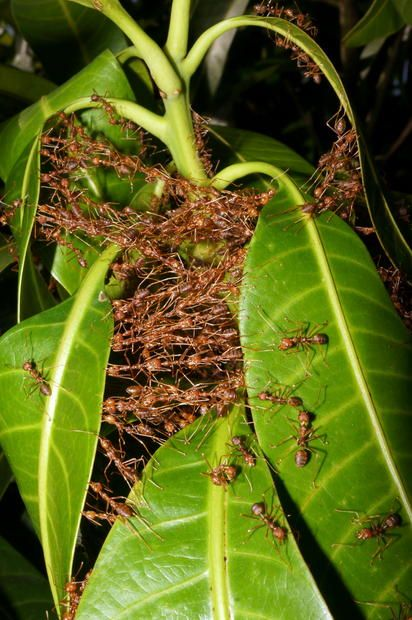
\includegraphics[height=40mm]{fig/cap02/hormiga_tejedora.jpg}}\hspace{3cm}
    \subcaptionbox{Tejiendo dos hojas\label{fig:hormiga-tejedora-b}}{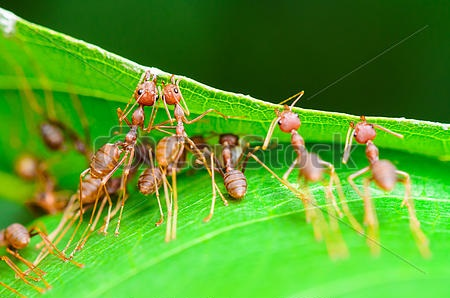
\includegraphics[height=40mm]{fig/cap02/oecophylla-tejiendo.jpg}}
\caption{Hormiga tejedora (\textit{Oecophylla})} 
\label{fig:Figura_HormigaTejedora}
\end{figure}

Las abejas por su parte, organizan sus colmenas en paralelo formando cadenas que inducen a un aumento de temperatura permitiendo así que sea más fácil moldearlas, como es el caso de la especie (\textit{Apis mellifica}) tal y como se puede observar en la figura \ref{fig:Figura_EnjambreAbeja}. En ciertos momentos la colonia se divide de tal forma que la abeja reina y la mitad aproximadamente de las trabajadoras abandonan la colmena formando un grupo en una rama cercana. Las exploradoras por su parte, exploran cuidadosamente los sitios potenciales de anidación pudiendo durar este proceso de selección varios días.

\begin{figure}[!ht]
\centering
    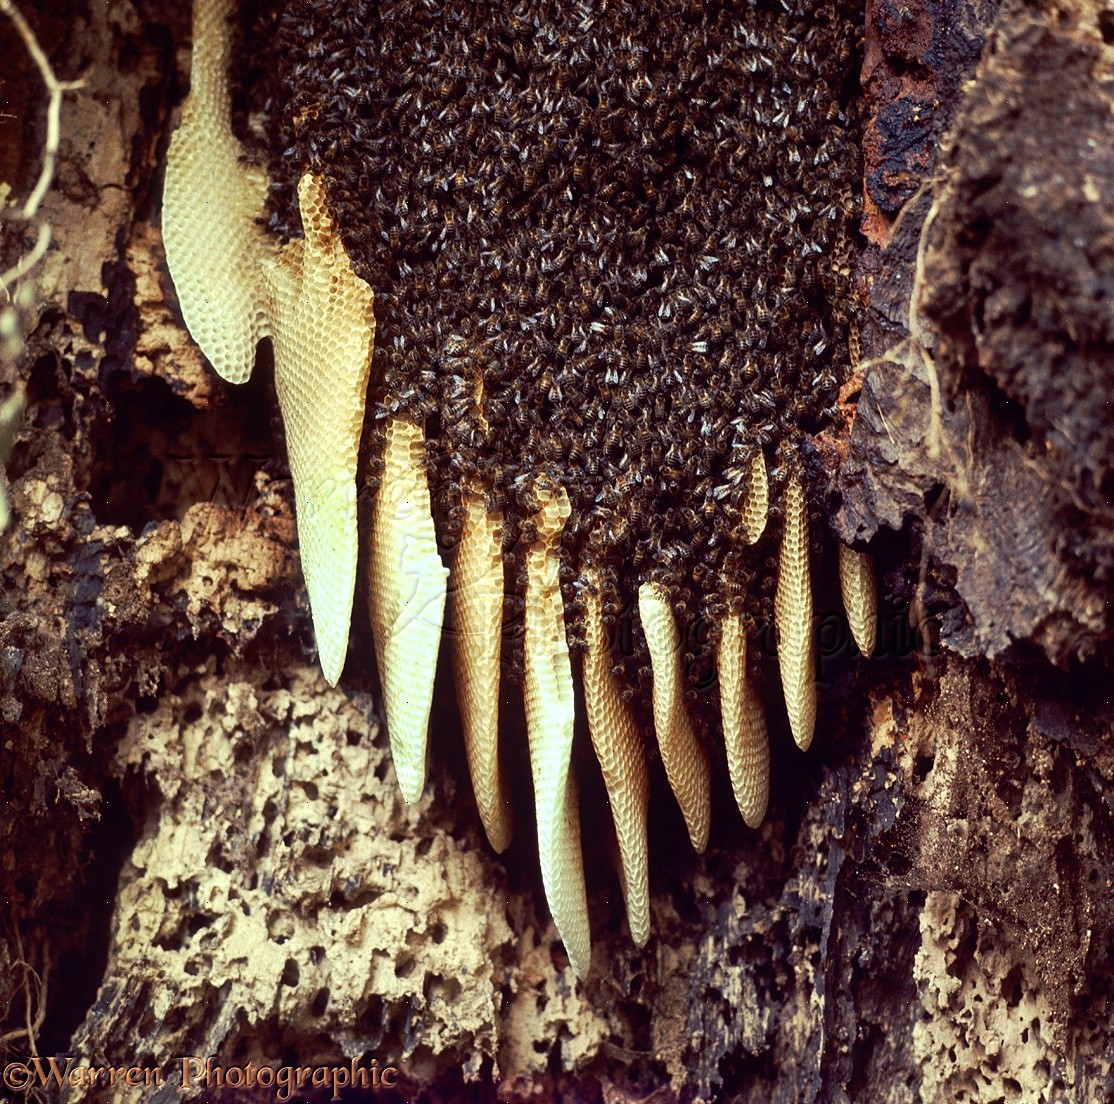
\includegraphics[height=6cm]{fig/cap02/Honey-Bee-comb.jpg}
    \caption{Enjambre de abejas \textit{Apis mellifica}}
    \label{fig:Figura_EnjambreAbeja}
\end{figure}

Estos tipos anteriormente descritos de comportamiento en insectos sociales son referentes a la organización de las tareas del grupo, en función de las características de cada individuo con una finalidad clara de mejorar la productividad. Se pueden leer más ejemplos de insectos sociales en las referencias \cite{csahin2004swarm,robinson1992regulation}. 

Existe otro tipo de comportamiento colectivo, que hace referencia a la dinámica del grupo que se observa en bandadas de pájaros, manadas de animales o bancos de peces, entre otros. Éste hace referencia al comportamiento individual de cada animal que les permita coordinar sus movimientos en relación a los demás integrantes del grupo. Existen numerosos artículos y estudios sobre el comportamiento de los peces y la formación de bancos de peces (\textit{Schooling})\footnote{Según I. Aoki: ``Resultado de las interacciones en las que un individuo controla su movimiento en relación con los vecinos y, al mismo tiempo, influye en estos vecinos"} dependiendo de diferentes factores externos. Una pequeña muestra de artículos relacionados con esta rama de estudio son \cite{aoki1982simulation, Aoki1984experimental,hall1910hidden,partridge1980sensory,partridge1980three,Pitcher963blindfish,youseff2008parallel}. 

Aoki, en su artículo \cite{aoki1982simulation} estudia el comportamiento de cada individuo del banco en función de la distancia del vecino más cercano. Para ello, basó sus estudios en un principio de la organización de los bancos de peces que estableció Edward T. Hall \cite{hall1910hidden}, según el cual el comportamiento depende tanto de la distancia personal como de la distancia social y se encontró con que los movimientos grupales podrían ocurrir a pesar de que cada individuo careciese de conocimiento del movimiento de todo el banco y en ausencia de un líder consistente. Esto podía ocurrir si individualmente llevaban a cabo tanto un movimiento de aproximación que permitiera la agregación como un movimiento de orientación paralela para que el banco mantuviera la cohesión.

Atendiendo en esta ocasión al comportamiento de las aves, estas bandadas naturales parecen basar su movimiento en dos comportamientos opuestos y equilibrados: el deseo de permanecer cerca de la bandada y el deseo de evitar colisiones entre cada ave. Pero aunque la razón por la que desean evitar colisiones parece evidente, ¿por qué deciden permanecer unidos a pesar de que sería más fácil el vuelo por separado?. El impulso básico de las aves para unirse a una bandada es el resultado de la presión evolutiva de varios factores como la protección contra los depredadores, una búsqueda más fácil de alimentos aumentando el patrón de búsqueda o las ventajas para las actividades sociales y de apareamiento. Esto lo trata \citeauthor{reynolds1987flocks} en su artículo \cite{reynolds1987flocks} y más adelante se tratará con más profundidad en este trabajo.

\begin{figure}[!ht]
    \centering
    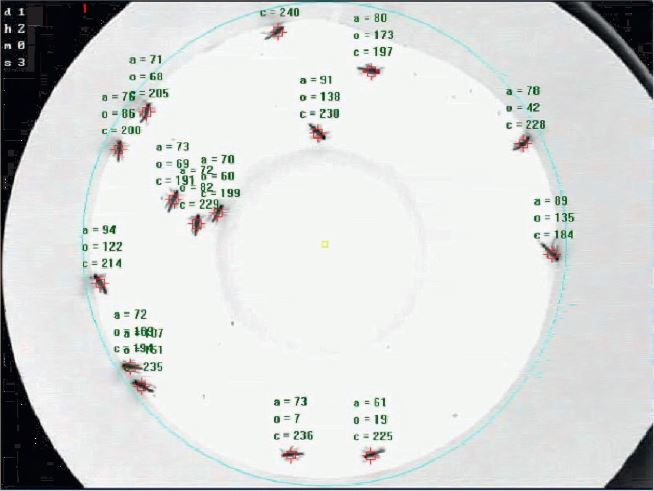
\includegraphics[height=8cm]{fig/cap02/Locusts.JPG}
    \caption{Langostas en el Sombrero Mexicano monitorizadas con el software que utilizó \citeauthor{buhl2006disorder} en sus estudios}
    \label{fig:locust_mexican_hat}
\end{figure}

\citeauthor{buhl2006disorder}\cite{buhl2006disorder} hicieron un estudio sobre las langostas en el que observaron que las juveniles se agrupaban fácilmente en bandas de marcha altamente coordinadas en condiciones de laboratorio, cuando las colocaron en un terrario en forma de `sombrero mexicano'. Los individuos seleccionaron colectivamente una dirección de movimiento en sentido horario o en sentido antihorario aleatoriamente y mantuvieron esto durante períodos prolongados. El movimiento de las langostas se registró durante ocho horas y los datos resultantes se procesaron utilizando el software de seguimiento para calcular la posición y orientación de cada langosta (véase la figura \ref{fig:locust_mexican_hat}). \citeauthor{buhl2006disorder} llegaron a la conclusión de que este comportamiento dependía en gran medida de la densidad de población en el sombrero. A mayor densidad, mayor era la alineación de los movimientos en el grupo.


Aunque el efecto de agregación en animales es obvio y claramente visible al ojo humano (peces, aves, insectos...) el análisis heurístico únicamente basado en lo que vemos no es suficiente para responder a la pregunta fundamental de cómo y por qué ocurre esto. Parrish analiza en conjunto los estudios anteriores en busca de similitudes y diferencias entre los diferentes algoritmos, identificando la relación entre el comportamiento individual de cada individuo y el del conjunto del grupo en \cite{parrish2002self}. 

En un principio, Parrish identifica dos maneras de ver la integración de los animales en un grupo; por una parte, existen animales territoriales con poca necesidad de participar en la transferencia de información y sin necesidad de estructura grupal y por otra, la que interesa desde el punto de vista del \textit{Swarming}, se encuentran las asociaciones altamente integradas a largo plazo. En las segundas tienen lugar altas tasas de intercambio de información, están compuestas por individuos que se conocen y están relacionados con otros miembros, siendo evolutivamente más beneficiosos ya que el contacto sensorial entre individuos es el reflejo de las condiciones ambientales o morfologías de los organismos.

Los estudios que se han hecho hasta el momento han sido en condiciones muy artificiales, generalmente con un número reducido de individuos debido a la dificultad de recoger datos fiables. Por ejemplo, en el caso de la observación de un banco de peces, es fácil entender la complejidad a la que se exponen los investigadores debido a que por una parte, se realizan en un medio acuático y por otra parte, hay peces más profundos en el mismo banco que no se ven desde la superficie e intervienen igualmente en el movimiento colectivo. Por tanto, mientras las técnicas de observación de estos animales no avancen, es difícil obtener una relación entre el comportamiento de un pez y el grupo. Parrish recoge los datos de los estudios anteriores más relevantes para compararlos entre ellos, aunque cada uno contenga datos relativamente diferentes. Tras la comparación se puede observar que no siempre se consigue el consenso en la dirección de los peces del banco. En la tabla \ref{tab:tablaRaynolds} se recogen algunos de todos los que Parrish compara en su artículo.

\begin{center}
\begin{spacing}{0.5}
    \small{
    \begin{table}[t]%[h!]
        \begin{tabularx}{1\textwidth}{>{\raggedright\arraybackslash}X >{\raggedright\arraybackslash}X >{\raggedright\arraybackslash}X >{\raggedright\arraybackslash}X >{\raggedright\arraybackslash}X} 
            \hline
            Referencia & Tamaño de la población & Orientación de partida & Velocidad & ¿Consenso?\\  
            \hline\hline
            Aoki (1982,1984) & 8,32 & Posición aleatoria y orientación dentro de área delimitada & Aleatoria & Sí\\ 
            \hline
            Warburton y Lazarus(1991) & 2-9 & Rejilla cuadrada & Sin especificar & No\\
            \hline
            Huth y Wissel (1990-92-94)& 8 & Posición aleatoria y orientación en área fija & Aleatoria & Sí\\
            \hline
            Reuter y Breckling (1994) & 10, 20, 30, 40, 50 & Posición aleatoria y orientación dentro de área delimitada & Difusa & Sí\\
            \hline
            Romey (1996) & 2-10 & Posición aleatoria y orientación dentro de área delimitada & Constante & No\\
            \hline
            Vab{\o} y N\o ttestad (1997) & 900 & Posición aleatoria y orientación dentro de área fija y delimitada & Constante & No\\ 
            \hline
            Stocker (1999) & 12, 64 & Posición aleatoria y orientación dentro de área delimitada & Constante & Sí\\ 
            \hline
            
        \end{tabularx}
        \caption{Tabla de Reynolds comparativa de los diferentes estudios}
        \label{tab:tablaRaynolds}
    \end{table}
    }
\end{spacing}
\end{center}

\newpage
\clearpage

\subsection{Auto-organización en la robótica} \label{s2_1_2}

La estructura organizativa que tienen los animales vistos hasta ahora tiene un gran beneficio si lo aplicamos a los enjambres de robots \footnote{\textit{Swarm robotics}: La robótica de enjambre es el estudio del diseño de un gran número de agentes físicos relativamente simples de modo que el comportamiento colectivo deseado surja de las interacciones locales entre los propios agentes y entre los agentes y el medio ambiente.\cite{csahin2004swarm}}. Hoy en día cada vez son más las tareas que tienden a automatizarse y para muchas de ellas son necesarios un grupo de robots. Además, las propiedades que caracterizan un sistema auto-organizado, como la escalabilidad, la flexibilidad y la robustez, también son muy deseables para un enjambre de robots autónomos. Es debido a esta creciente importancia que este enfoque merece ser explicado. En \cite{christian2008swarm} los autores introducen un estudio de este concepto antes de presentamos una breve revisión de la investigación en robótica de enjambres a lo largo de cuatro ejes: diseño, modelado y análisis, robots y problemas.

Son las tres características mencionadas anteriormente las que usa como nexo de unión entre la auto-organización aplicada a la biología y a la robótica: 

\begin{itemize}
    \item \textbf{Robustez}: en los enjambres la pérdida de un individuo puede ser inmediatamente compensada por otro, la coordinación está descentralizada y, por lo tanto, es poco probable que la destrucción de una parte particular del enjambre detenga su operación, la simplicidad de los individuos los hace menos propensos al fracaso y la percepción sensorial se distribuye y por tanto, el sistema es robusto frente a las perturbaciones locales del entorno.
    \item \textbf{Flexibilidad}: los individuos de un enjambre deben ser capaces de coordinar sus comportamientos para abordar tareas de diferente naturaleza.
    \item \textbf{Escalabilidad}: debe poder operar en una amplia gama de tamaños de grupo y apoyar a una gran cantidad de individuos sin afectar considerablemente el rendimiento.
\end{itemize}

A estas características los autores añaden otras que debe tener el enjambre como tener una forma y masa y ser capaces de interactuar físicamente con su entorno, ser idénticos al menos en la manera de interactuar, ser capaces de realizar la tarea con la mayor simpleza posible y tener habilidades de interacción local. Además cabe destacar que dos de los principales mecanismos de coordinación que funcionan en los sistemas naturales son válidos para los sistemas robóticos y son la auto-organización y la estigmergia \footnote{\textit{Estigmergia}: en biología, se refiere a la capacidad que tienen algunos sistemas descentralizados de contribución a través del medio que los rodea} (se puede leer más sobre este término en \cite{estigmergia1} y \cite{estigmergia2}). 

Una vez sentadas las bases teóricas sobre las características que deben tener un enjambre de robots, \citeauthor{christian2008swarm} recorren lo que ellos consideran son las líneas de investigación para poder desarrollarlo. 

En cuanto al diseño, agrupa los estudios en en función de si lo que se busca es que cumpla una funcionalidad o \textit{ad-hoc} o que se diseñe en base a unos principios. Un diseño ad-hoc asume implícitamente que el enjambre el grupo de robots va a tener un comportamiento similar a los insectos o animales utilizados como inspiración. En el diseño basado en principios en lugar de diseñar un comportamiento específico a nivel de enjambre, se utiliza una metodología general a través de la cual se pueden usar los comportamientos deseados a nivel de enjambre para construir los comportamientos individuales necesarios.

Otra linea de investigación es el modelado y análisis, para lo cual divide 3 tipos diferentes de modelado. El primero, basado en sensores, es utilizado principalmente para construir simuladores realistas de sistemas robóticos y nos permite realizar experimentos en simulación y así obtener resultados que se aproximan en mayor medida con los obtenidos de los robots físicos. En segundo lugar, existe el modelado microscópico que tiene en cuenta las características del entorno, la forma física y el control del comportamiento de los robots de tal manera que a la vez que simula las interacciones individuales dentro del sistema, también es capaz de adaptar los estados individuales en el tiempo. Por último, el modelado macroscópico simula el comportamiento de unas cantidades medias que representan el estado del sistema. Este último es común en física y química y es suficiente con resolverlos solo una vez para obtener el estado estacionario del modelo.

Otra de las principales líneas de investigación ha sido el desarrollo de enjambres de robots físicos, ya que la construcción de un sistema robótico requiere más que reunir una cantidad de copias de una plataforma robótica genérica. Todos los estudios con este fin se han centrado en el desarrollo de robots móviles que tienen como objetivo proporcionar una plataforma de investigación y no están destinados a la operación en el mundo real. A los ya mencionados con anterioridad existen una serie de requisitos adicionales que deben tener estos sistemas físicos desde el punto de vista de los investigadores que tienen que ver con la detección y señalización de los propios robots, la comunicación, la interacción física entre ellos y con el entorno, la fuente de energía de la que disponen y cómo la utilizan, el costo de producción y de puesta en marcha, el tamaño o tener simuladores.

Esta última aplicación de enjambres de robots, aún se encuentra en una fase muy inicial de desarrollo pero sin lugar a duda, es la que presenta el mayor potencial de aplicación para el futuro de la robótica.


\section{Modelos matemáticos} \label{s2_2}
Para comprender el contexto de los modelos matemáticos que estudian el comportamiento colectivo, 

Los modelos matemáticos que estudian el comportamiento colectivo encuentran una fuerte base en los modelos clásicos que han servido históricamente para estudiar el crecimiento de conjuntos de poblaciones.

\subsection{Modelos clásicos poblacionales} \label{s2_2_1}
En este apartado, hay 3 modelos clásicos que requieren una breve explicación:

\subsubsection{Modelo de Malthus}
En su artículo \cite{malthus1846ensayo} quería demostrar que nuestro crecimiento es insostenible y acabaría desembocando en una pauperización y en una economía de subsistencia, si no directamente en la extinción. Malthus utiliza el modelo de crecimiento exponencial del Carbono 14 para emular el crecimiento poblacional, es decir, cada año la población aumenta o disminuye un cierto tanto por uno $p$ respecto a lo que había el año anterior según la siguiente fórmula:

\begin{equation}
    N_{k} = N_0\cdot C_k \quad \textrm{donde} \quad C = (1+\Delta tR_0)
\end{equation}

\noindent que si lo pasamos al modelo continuo haciendo tender $\Delta t -> 0$ queda:

\begin{equation}
    N'(t) = C \cdot N(t) => N(t) = N_0 \cdot e^{Ct}
\end{equation}

\subsubsection{Modelo Logístico}
Tras leer el ensayo de Malthus, Pierre-Fran\c{c}ois Verhulst \cite[Cap.~37,38]{haberman1998mathematical} publica un nuevo modelo basándose en el de su predecesor, pero añadiendo que la tasa de reproducción es proporcional tanto a la población existente como, además, a la cantidad de recursos disponibles, asumiendo así que existe un punto de saturación el cual significa que si la población crece mucho, entonces te quedas sin recursos para abastecerla y por tanto deja de crecer. Según esto, el modelo Logístico discreto que propone Verhulst queda de la siguiente forma:

\begin{equation}
    \displaystyle{\frac{\Delta N}{\Delta t} = (C_1 \cdot N_k) \cdot (C_2 \cdot (1-N_k)}
\end{equation}

\noindent que agrupando algunas de las constantes y re-escalando la unidad de medida del número de individuos se obtiene:

\begin{equation}
    N_{k+1} = C \cdot N_k \cdot (1 - N_k)
\end{equation}

\noindent cuya solución del modelo continuo quedaría:

\begin{equation}
    \displaystyle{N(t) = \frac{\frac{a}{b}}{1+(\frac{a-bN_0}{bN_0})e^{-at}}} 
\end{equation}

Una evolución de este modelo sería el que propone Lotka Volterra \cite[Cap.~43]{haberman1998mathematical} que lo aplica a dos sistemas coexistentes, de los cuales uno es el sistema depredador y otro es el sistema presa estando estrechamente relacionado la evolución de ambos.


\subsection{Modelo de Keller-Segel} \label{s_2_2_2}
Otro modelo matemático de importancia es el presentado por Evelyn Fox Keller y Lee A. Segel \cite{keller1970initiation, keller1971model, keller1971traveling}, que estudian el comportamiento de insectos cuyos comportamientos y movimientos los llevan a cabo de acuerdo a unos gradientes de sustancias químicas. Este modelo ha sido muy utilizado en diversos ensayos, algunos de los cuales más importantes pueden leerse en las referencias \cite{calvez2008parabolic, blanchet2008convergence, calvez2006volume, dolbeault2004optimal, blanchet2006two, corrias2006critical}.

En el libro \textit{Swarm intelligence: from natural to artificial systems}, \citeauthor{bonabeau1999swarm} estudian patrones en dos insectos diferentes: hormigas y termitas. Las primeras, utilizan la temperatura y humedad del ambiente para construir sus nidos y distribuyen sus crías en función de eso. Las segundas, por su parte, construyen la cámara real adaptándola al cuerpo de la reina y la forma y el tamaño de la cámara la define el gradiente de feromonas que desprende a su alrededor. De esta manera la reina crea una plantilla química.

Las termitas empiezan construyendo la cámara por los pilares. La disposición general de los gránulos y por tanto de la aparición de éstos queda descrita por el sistema de ecuaciones \eqref{eq:PhoromoneConcentration}-\eqref{eq:activeMaterialDyn},
que definen la concentración de la feromona en un punto y momento, la densidad de las terminas trabajando y la dinámica del material disponible. Estas ecuaciones se forman a partir de parámetros como: producción total en función de la cantidad de feromonas, flujo de paso de las termitas al lugar de construcción, movimiento aleatorio de cada termita o capacidad de atracción de la feromona entre otros. 

\begin{equation}\label{eq:PhoromoneConcentration}
    \delta_{t}H = k_{2}P-k_{4}H+D_{H}\nabla^{2}H
\end{equation}
\begin{equation}\label{eq:termitesDensity}
    \delta_{t}C = \Phi-k_{1}C+D_{C}\nabla^{2}C-\gamma\nabla(C\nabla H)
\end{equation}
\begin{equation}\label{eq:activeMaterialDyn}
    \delta_{t}P = k_{1}C-k_{2}P
\end{equation}

La concentración de feromonas ($H$) se determina en función de la producción total de feromonas ($k_{2}P$) la disminución de feromonas ($-k_{4}H$) y de la difusión de feromonas ($D_{H}\nabla^{2}H$) según se muestra en la ecuación \eqref{eq:PhoromoneConcentration}. Por otra parte, la densidad de las termitas trabajando, $C$, es definida por la ecuación \eqref{eq:termitesDensity} dependiente del flujo de paso de las termitas con gránulos a la zona de construcción ($\Phi$), la tasa de descarga de termitas por unidad de tiempo ($-k_{1}C$), $D_{C}\nabla^{2}C$ que es el componente aleatorio que define el movimiento de las termitas y la capacidad de atracción de la feromona mediante $\gamma\nabla(C\nabla H)$. La última variable que influye en la disposición y organización de granos es la dinámica del material disponible (ecuación (\ref{eq:activeMaterialDyn})) definido por la cantidad de P que sería igual que $-k_{1}C$ y el ratio de desaparición del material disponible ($-k_{2}P$).

Este estudio concluye que a mayor acumulación de granos, hay mayor acumulación de termitas y mayor será por tanto la acumulación de feromonas en un mismo punto, lo cual genera un efecto \textit{bola de nieve} que atraerá más termitas con granos para formar pilares, lo que conlleva a una construcción de pilares homogénea y regular en el espacio (figura). A estas ecuaciones, \citeauthor{deneubourg1977application} \cite{deneubourg1977application} y \citeauthor{bruinsma1979analysis} \cite{bruinsma1979analysis} añaden ecuaciones más complejas en las que analizan el potencial de las feromonas de la reina. A partir de este ejemplo, se ve que la combinación de auto-organización y una plantilla exhibe las propiedades de la auto-organización, como el efecto bola de nieve, y al mismo tiempo produce un patrón perfectamente predecible, la cámara real que está formada por muros construidos. siguiendo la plantilla feromonal de la reina.

\begin{figure}[h!]
    \centering
    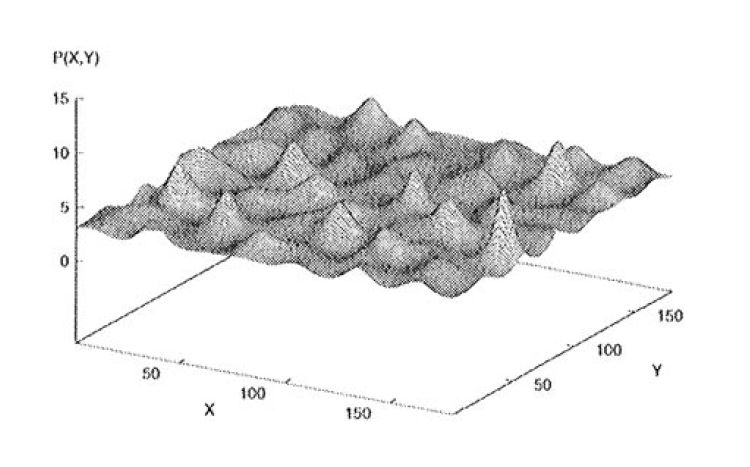
\includegraphics[height=7cm]{fig/cap02/distrubucionPilaresTermitas.JPG}
    \caption{Distribución de los pilares para la construcción de la cámara real de las termitas}
    \label{fig:pillarsTermites}
\end{figure}

\subsection{Modelos basados en agentes}\label{s2_2_2}
Basando sus estudios en la observación de un banco de peces, Aoki parte de dos premisas principales: que la velocidad y dirección de cada individuo son variables estocásticas y se determina otros principios como que el tiempo se cuantificaba como \(\Delta T\) o que el organismo se mueve en dos dimensiones. Adicionalmente, para simplificar el problema limita la interacción entre los individuos al componente direccional y el componente velocidad pasa a determinarse independientemente de los otros elementos del grupo \cite{aoki1982simulation}. 

\begin{figure}[!h]
    \centering
    {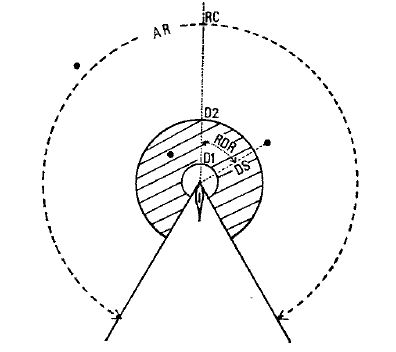
\includegraphics[height=6cm]{fig/cap02/movimientoPecesAoiki.JPG}}
    \caption{Ilustración con los parámetros que influyen en el modelo de Aoki}
    \label{fig:aokiFishInteractions}
\end{figure}\label{fig:aokifish}

Tomando como referencia el esquema representado en la figura \ref{fig:aokifish} y partiendo de las premisas anteriormente expuestas, Aoki define los siguientes modelos matemáticos para definir la distribución de la velocidad:
\begin{equation}\label{eq:velocityDistributionAoki} 
    f(v) = \displaystyle{\frac{A^{K}}{\Gamma (K)}}e^{-Av}v^{K-1}
\end{equation}

\noindent y la probabilidad de alineación en la dirección \(p_{i}(\theta)\):
\begin{equation}\label{eq:directionDistributionAoki}
    p_{i}(\theta)=\sum_{j}W_{j}\frac{1}{S_{j}\sqrt{2\pi}}e^{-(\theta -M_{j})^2/2S_{j}^2} 
\end{equation}


En la ecuación \ref{eq:velocityDistributionAoki} se encuentran  \(\upsilon\) como valor de la velocidad, \textit{K} y \textit{A} como parámetros constantes y mayores que cero y \(\Gamma(K)\) que es una función gamma. En la segunda ecuación (\ref{eq:directionDistributionAoki}) \(W_{j}\) es el factor que pondera la influencia que tiene cada individuo dentro de la distancia \textit{RC}. 

La dirección del movimiento está pues, relacionada con la ubicación y el rumbo de los vecinos. La influencia que ejercen los individuos entre sí se define mediante la ecuación$$ W_{j+1}=RF \cdot W_{j},$$ donde \textit{RF} es una constante entre 0 y 1 definida para cada simulación. Todo esto conlleva a establecer que los individuos pueden tener tres tipos de conductas diferentes dentro del grupo en función de las distancias y las interacciones que tienen: aproximación, sorteo/evitación y orientación paralela.

El modelo descrito anteriormente se programó para realizar los cálculos necesarios, y se ejecutó siguiendo un algoritmo muy bien definido que se muestra en el flujo de figura \ref{fig:flowchartAoki}. Tras ejecutar su modelo numerosas veces cambiando los parámetros de entrada, llegó a la conclusión de que a lo largo de las 2000 iteraciones de cada ejecución, los individuos permanecían en grupo mostrando siempre comportamientos muy similares. 

\begin{figure}[h!]
    \centering
    {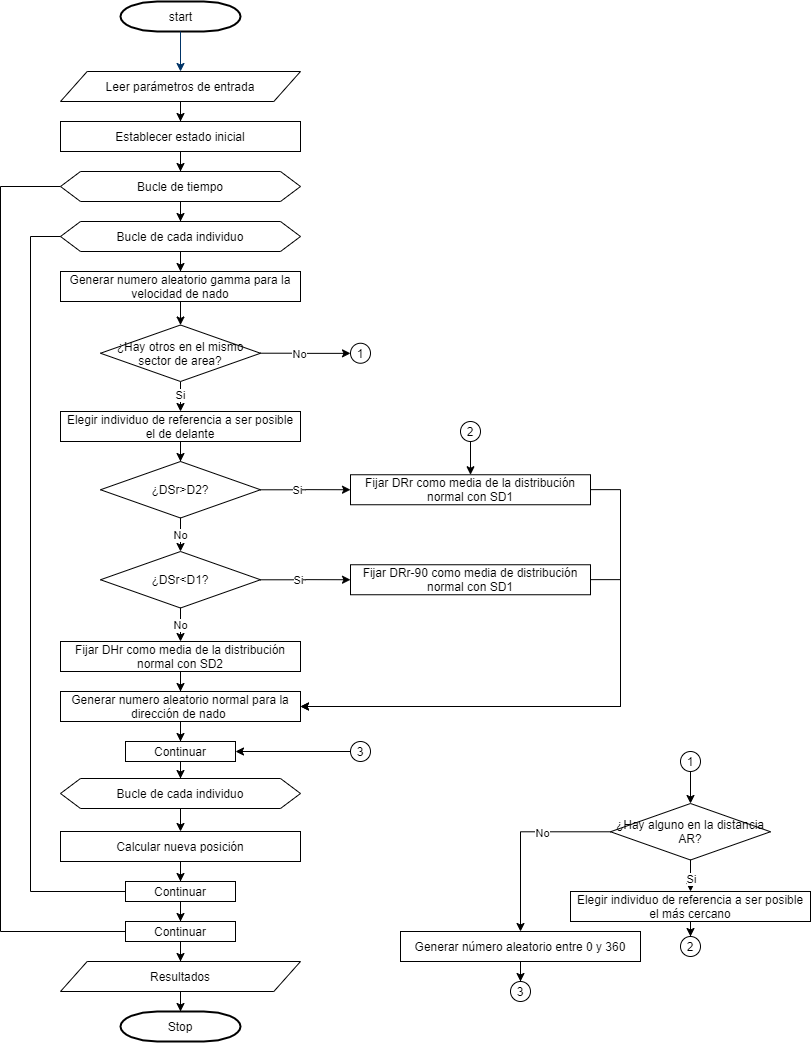
\includegraphics[height=15cm]{fig/cap02/AlgoritmoAoki.png}}
    \caption{Diagrama del flujo del modelo de simulación de Aoki}
    \label{fig:flowchartAoki}
\end{figure}

Estos estudios que inició Aoki, en los que simplifica el modelo con premisas iniciales para poder optimizar las simulaciones, dieron lugar a la exploración desde distintos enfoques de las propiedades de comportamiento con las que están dotadas las especies gregarias como los peces. En estudios posteriores se incluyen la limitación de una pista sensorial para estudiar el cambio de comportamiento \cite{partridge1980sensory,Pitcher963blindfish}, el estudio de las reacciones a objetos estacionarios o móviles \cite{shaw1971optomotor} o el análisis de movimientos individuales y se siguió concluyendo que los movimientos grupales en la unidad podían ocurrir a pesar de carecer cada individuo del conocimiento del movimiento de todo el banco de peces.

Otro estudio, mencionado en un punto anterior, realizado en esta ocasión por Reynolds, se centra en encontrar un modelo óptimo para poder simular el movimiento de una bandada de pájaros en una animación por ordenador \cite{reynolds1987flocks}. Parte de la problemática inicial que tienen otros modelos es la dificultad de simular el movimiento real de animales colectivos ya sean bandada de pájaros, manadas de animales, banco de peces o cualquier grupo dentro del espectro que conocemos y estamos tratando como animales colectivos.

En este estudio, Reynolds se centra en bandadas de pájaros y propone que no es imposible simular el movimiento de un grupo de aves por ordenador, pero se necesita un mejor enfoque para una animación eficiente, robusta y creíble. Para ello el modelo se enfoca desde la suposición de que una bandada es simplemente el resultado de la interacción entre los comportamientos individuales de las aves.

Según el autor, ``el movimiento general parece fluido; tiene un concepto simple, pero es tan visualmente complejo que parece aleatoriamente organizado y, sin embargo, está magníficamente sincronizado'' y es por ello que traslada estos movimientos a un enfoque geométrico.

En un vuelo real, los giros y movimientos ocurren de forma continua y simultánea. Por su parte el vuelo geométrico incremental que propone es una aproximación discreta de esto; pequeños movimientos lineales que modelan una trayectoria curva continua. En términos cartesianos, el eje derecha-izquierda es X, arriba / abajo es Y, y adelante-atrás es Z (ver figura \ref{fig:geometricalFlight}). Adicionalmente a esto, para modelar el vuelo hay que tener en cuenta la gravedad contrarrestada con la flotabilidad del ave por el efecto de las alas.

\begin{figure}[h!]
    \centering
    {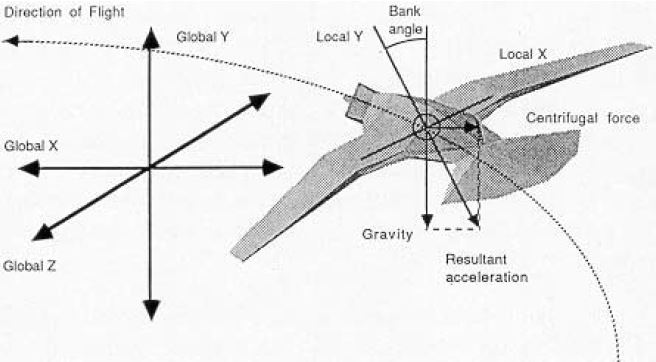
\includegraphics[height=5cm]{fig/cap02/geometricalFlight.JPG}}
    \caption{Geometría del vuelo de Reynolds}
    \label{fig:geometricalFlight}
\end{figure}

Para que se formen las bandadas, cada individuo debe tener comportamientos que permitan la coordinación con los de sus compañeros, que en contra de lo que parece, no son totalmente aleatorios, si no que tienen movimientos comunes.

Un ave puede ser consciente de tres factores: de sí mismo, sus de 5 a 7 de sus vecinos más cercanos \cite{ballerini2008interaction}\footnote{En un principio Reynolds contempla que le influye el comportamiento de sus 2 o 3 vecinos más cercanos, pero es Ballerini et al. quienes demuestran que el número de vecinos está entre 5 y 7.} y el resto de la bandada. Es por esto por lo que una bandada de pájaros no tiene límite de individuos y nunca parece estar sobrecargada ya que la cantidad de factores que un mismo ave tiene que tener en cuenta para mantenerse en la bandada es independiente del número de individuos que la integren. De esta manera, la tarea de volar siempre es igual de simple (o compleja).

Aunque el vuelo en bandada descrito anteriormente resulte aparentemente sencillo, el trabajo requerido para ejecutar el algoritmo en ordenador crece como el cuadrado de la población del rebaño y definitivamente existe un límite superior en el tamaño de las bandadas simuladas implementadas.

\subsection{Modelos de consenso}\label{s2_2_3}

En un contexto en el que cada vez más se tiende a estudiar el comportamiento de los animales para dar respuesta al por qué del movimiento y comportamiento de los animales para poder simularlo e incluso contemplar la posibilidad de imitarlo en el ser humano, no es hasta 1995, cuando Vicsek realiza un estudio bastante simple basado en dos ecuaciones que veremos a continuación. Con tal de imitar la dinámica de movimiento y explicar el consenso de ciertos sistemas, define para sus partículas un impulso inicial con una velocidad absoluta constante y en cada paso de tiempo cada individuo asume la dirección promedio de sus vecinos en un radio establecido \cite{vicsek1995novel}. Basándose en estas asunciones, Vicsek es capaz de demostrar matemáticamente que las simulaciones de movimientos auto-organizados pueden llevarse a cabo.

Para entender matemáticamente este modelo, la posición de cada \(i\)-ésima partícula viene dada por:
\begin{equation}\label{eq:vicsekParticlePosition}
    x_{i}(t+1)=x_{i}(t)+\mathbf{v}_{i}(t)\Delta t
\end{equation}
 donde la velocidad de la partícula $\mathbf{v}_{i}(t+1)$ se construye para tener un valor absoluto $v$ y una dirección dada por el ángulo $\theta (t+1)$ obtenido mediante la expresión: 
 \begin{equation}\label{eq:vicsekParticleDirection}
    \theta (t+1)=\langle\theta (t)\rangle _{r}+\Delta \theta
 \end{equation}
 donde $\langle \theta (t)\rangle _{r}$ es la dirección media de las del grupo que rodea a la partícula $i$ en un radio $r$. También en \ref{eq:vicsekParticleDirection} $\Delta \theta$ es un número aleatorio entre dos valores definidos $[-\mu /2 , \mu /2]$ que representa la perturbación por algún agente externo. 
 
 El resto de su estudio se basa en comprobar el comportamiento que tienen las partículas en base a los dos parámetros básicos, el ruido $\mu$ y la densidad $\rho = N/L^{2}$. Modificando estos valores se da cuenta de que siempre hay consenso entre las partículas en mayor o menor medida. Para densidades y perturbaciones pequeñas, las partículas tienden a formar grupos moviéndose cada uno guardando cierta cohesión. Cuando la densidad y el ruido son muy altos todas las partículas tienden a llevar la misma dirección aunque sea aleatoria. El caso más interesante es cuando la densidad es elevada y la perturbación es baja, en cuyo caso el movimiento se lleva a cabo de manera ordenada a nivel macroscópico. 
 
 Un trabajo de investigación muy interesante que surge a raíz del modelo de Vicsek, es el realizado por Alethea Barbaro y un grupo de científicos y biólogos, en el cual aplica el modelo a la población de capelán islandés para reproducir la ruta de migración durante tres años diferentes, prediciendo con éxito la ruta para 2008 \cite{barbaroModellingSimulations}. El valor de este estudio radica en que en ese año predijeron que llegarían a un lugar donde nunca habían estado. Utilizando los datos de temperatura disponibles y las corrientes aproximadas, pudo reproducir las rutas migratorias observadas de los tres años anteriores \cite{barbaro2009simulations}. Primero se hizo un análisis para identificar la temperatura oceánica y el equilibrio entre la influencia de la interacción entre partículas y la respuesta de las partículas a la temperatura como los parámetros de control más significativos de cara a determinar la ruta de migración.
 
 Otros dos autores que dedican gran parte de su investigación a buscar un modelo de consenso son Felipe cucker y Steve Smale.  Aunque parten de los estudios de Vicsek, la diferencia con éste es que Cucker-Smale (C-S a partir de ahora) calcula la velocidad definiendo primero el vector de posición. Esto es así debido a que en un primer momento observaron que cualquier ``rebaño'' de animales, para el ejemplo me referiré a pájaros, terminan moviéndose a la misma velocidad sea cual sea su posición inicial. \cite{cucker2007emergent}.
 
 En este modelo, la velocidad de cada pájaro ajusta su velocidad añadiéndole una media ponderada de las diferencias de su velocidad con las de las otras aves. 
 
 \begin{equation}\label{eq:CSvelocidad}
     v_{i}(t+1)-v_{i}(t)=\sum_{j=1}^k a_{ij}(v_{j}(t)-v_{i}(t))
 \end{equation}
 
 Aquí, el valor del parámetro $\{a_{ij}\}$ cuantifica la manera en la que los pájaros influyen a los demás, que está relacionada con la distancia a la que se encuentran los pájaros sobre los que se ejerce esta influencia. Este valor también lo calculan mediante la ecuación 
 
 \begin{equation}
     \label{eq:CSaij}
     a_{ij} = \mu(||x_{i}-x_{j}||^2) = \frac{K}{(\sigma^2 + ||x_i-x_j||^2)^\beta}
 \end{equation}
 
 donde por cuestiones de simplicidad, se fijan los valores $K,\sigma>0$ y $\beta \ge 0$. Si se hace la derivada de la ecuación de la velocidad (\ref{eq:CSvelocidad}) obtendremos la función de la aceleración que ya se vio en el Capítulo 1:
 
 \begin{equation}
    \left\lbrace
    \begin{array}{ll}
        \dot{x}_{i}(t)=v_{i}(t) \\
        \dot{v}_{i}(t)= \displaystyle{\frac{1}{N}\sum_{j=1}^{N}\frac{v_{j}(t)-v_{j}(t)}{(1+||x_{j}(t)-x_{j}(t)||^2)^\beta}}
    \end{array}
    \right.
\end{equation}
 
Una de las características de este modelo es que el rebaño siempre llega a consenso sea cual sea su estado inicial, para valores de $\beta \leq 0,5$, correspondiente a una interacción a larga distancia social bastante fuerte. Por el contrario, para valores de $\beta >0.5$ el comportamiento de auto-organización se lleva a cabo bajo unas determinadas condiciones en el estado inicial, como por ejemplo, que el grupo en la posición inicial se encuentre lo más próximo al centro de masa del rebaño.

Para estos casos, si se quiere garantizar el consenso del grupo cuando no se cumplen estas condiciones iniciales, es necesario incluir estrategias de control al modelo, lo cual es el estudio del presente trabajo y se profundizará en el tema más adelante. 

A pesar de la elegancia de los resultados en cuanto a su comportamiento de consenso, la descripción de la dinámica auto-organizada por el modelo C-S sufre de varios inconvenientes que tratan de solucionar Sebastien Motsch y Eitan Tadmor proponiendo un nuevo modelo que no solo tiene en cuenta la distancia entre agentes, sino que también consideran la influencia que ejercen dos agentes entre sí en sus distancias relativas. Como consecuencia, lo que proponen Motsch y Tadmor no implica ninguna dependencia explícita del número de agentes sino que solo se tiene en cuenta su geometría en el espacio \cite{motsch2011new}. Los dos autores proponen en un primer momento el siguiente modelo: 

\begin{equation}
    \label{eq:MTmodel1}
    \left\lbrace
    \begin{array}{lll}
        \dot{x}_{i}(t)= v_{i} \\
        \dot{v}_{i}(t)=\displaystyle{\frac{\alpha}{\sum_{k=1}^{N}\phi_{ik}}\sum_{j=1}^{N}\phi_{ij}(v_{j}-v_{i})} \\ 
        \phi_{ij}=\phi(|x_{j}-x_{i}|)
    \end{array}
    \right.
\end{equation}

En este modelo, $\alpha$ es una constante positiva y $\phi$ es la función de influencia y la característica principal es que la influencia que ejerce el agente ``\textit{j}'' sobre el ``\textit{i}'' está ponderado por la influencia total del grupo $\sum_{k=1}^{N}\phi_{ik}$ ejercida sobre el agente ``\textit{i}''. Si todos los agentes están separados por la misma distancia, entonces este modelo tiende al de C-S, pero a diferencia de éste, la normalización de la interacción por pares entre agentes en términos de influencia relativa tiene como consecuencia la pérdida de simetría.

Por tanto, en agrupaciones grandes, si se pondera correctamente la influencia que ejercen todos los individuos de manera suficientemente lenta en función de la distancia a la que se encuentren, se consigue una cohesión del grupo independientemente de la configuración inicial, evitando de esta manera que sólo influya el comportamiento del vecino más cercano y llegando al consenso de manera mucho más efectiva.

 \subsection{Bertozzi y D'Orsogna}
 El siguiente modelo, propuesto por los autores \citeauthor{d2006self} en \cite{d2006self}, está basado en las- interacciones de atracción-repulsión:

\begin{equation}\label{eq:attractionRepulsion} 
    \left\lbrace
    \begin{array}{ll}
        \dot{x}_{i}(t)=v_{i}(t) \\
        \dot{v}_{i}(t)=\displaystyle{(\alpha - \beta |v_{i}|^{2})v_{i} -\frac{1}{N}\sum_{j\neq 1}\nabla U(|x_{i}-x_{j}|)}
    \end{array}
    \begin{array}{rr}
        (i = 1, ..., N) \\
        (i = 1, ..., N)
    \end{array}
    \right.
\end{equation}

$U$ representa el comportamiento de repulsión o de atracción entre los individuos, y puede definirse de diferentes maneras en función del control que se le quiera otorgar al modelo, por ejemplo, una elección típica es asignarle un valor: 

\begin{equation}\label{eq:potencialU}
    \left\lbrace
    \begin{array}{l}
        U(x) = k(|x|) \\
        k(r) = -C_{A}e^{-r/l_{A}}+-C_{R}e^{-r/l_{R}}
    \end{array}
    \right.
\end{equation}

donde $C_A$, $C_R$ y $l_A$, $l_R$ representan las fuerzas y longitudes típicas de atracción y repulsión respectivamente. Al depender de estos 4 parámetros, las posibilidades de comportamiento son muy diferentes, en función de los valores que se les asignen, por ejemplo, para valores $C_R = 50$, $l_R = 2$, $C_A = 20$, $l_A = 100$, $\alpha = 0.07$ y $\beta = 0.05$, encontramos que los individuos se organizan en una especie de remolino como en \ref{fig:remolino}. Sin embargo si a estos parámetros les asignamos los valores $C_R = 50$, $l_R = 20$, $C_A = 100$, $l_A = 100$, $\alpha = 0.15$ y $\beta = 0.05$ el resultado es que los individuos igualmente terminan formando un remolino, pero algunos de ellos en dirección a las agujas del reloj, mientras que otros, en sentido contrario. 

\begin{figure}[!ht]
\centering
    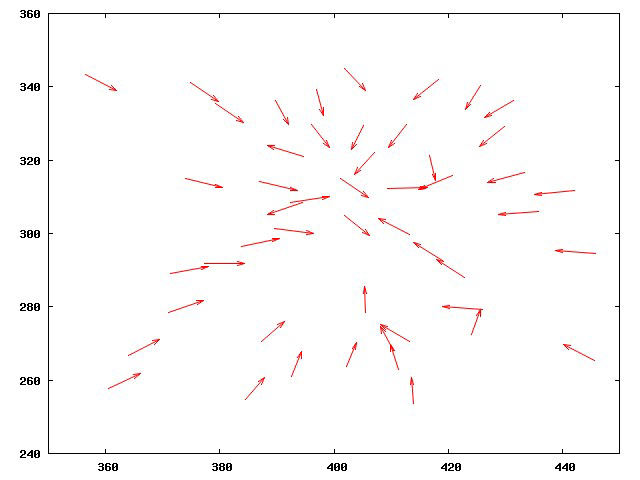
\includegraphics[scale=0.3]{fig/cap02/atraccionRepulsion/11.png}
    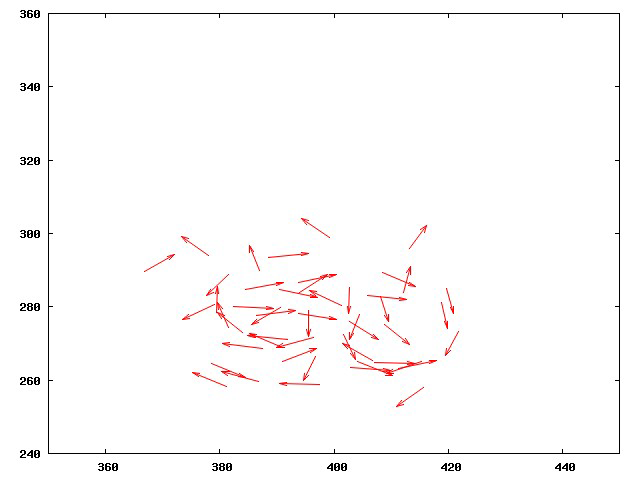
\includegraphics[scale=0.3]{fig/cap02/atraccionRepulsion/12.png}
    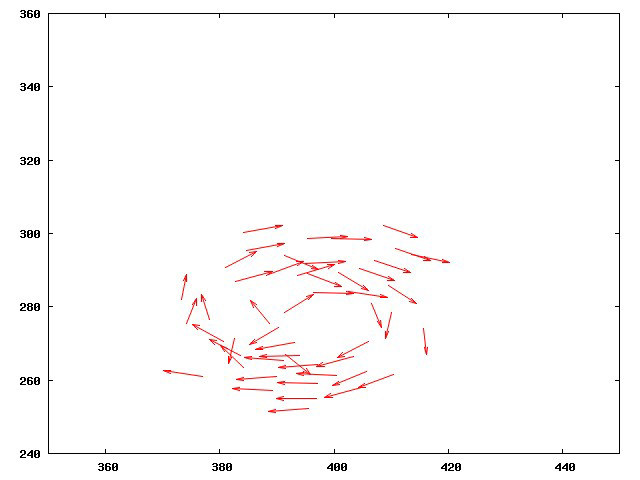
\includegraphics[scale=0.3]{fig/cap02/atraccionRepulsion/13.png}
    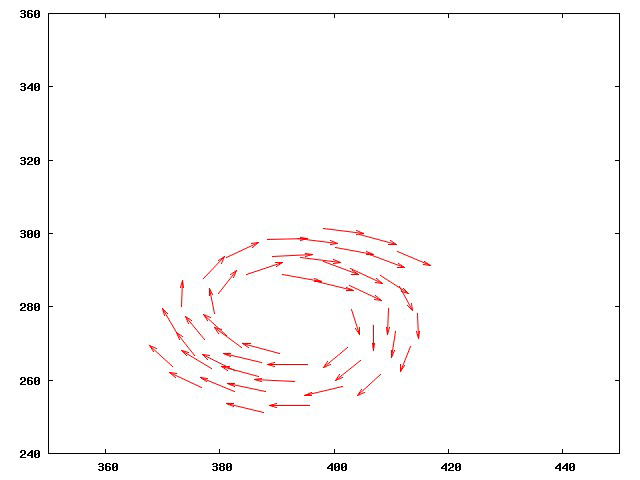
\includegraphics[scale=0.3]{fig/cap02/atraccionRepulsion/14.png}
\caption{Hormiga tejedora (\textit{Oecophylla})}
\label{fig:remolino}
\end{figure}

Por tanto concluyen en este estudio que el comportamiento del grupo puede controlarse exclusivamente con los parámetros $\alpha$, $\beta$, $C_A$, $C_R$ y $l_A$, $l_R$.
\chapter{Modelos de consenso mejorados} \label{cap3}

En este capítulo se abordarán los primeros estudios sobre swarming realizados por Cucker Smale así como los modelos de consenso mejorados que toman como referencia principal y añaden un control heurístico que afecta a alguna de las variables, para potenciar el consenso.%el de los primeros centrándose en mejorar algunas de las variables para modificar el modelo


\section{Introducción}\label{s3_1}
La auto-organización de grupos en los que no existe un líder es un comportamiento común de ciertos animales que comúnmente se han llamado sociales como pueden ser algunos insectos, peces o aves. Como se ha podido ver en el capítulo \ref{cap2}, dar una explicación matemática a este comportamiento ha supuesto siempre un reto difícil de resolver debido a la alta complejidad que supone comprender el comportamiento individual y colectivo de dichos seres vivos resultando en un campo de estudio que hoy en día se divide en varias vertientes.

Muchos de estos modelos se basan en el comportamiento individual de cada uno de los componentes del grupo, proporcionando para cada uno de ellos una ecuación para explicar la evolución de la posición, velocidad u otras características. Estos modelos se llaman `Modelos basados en individuos' (IBMs por su traducción al inglés \textit{Individual-Based Models}). Las estrategias de estos modelos son muy variadas y pueden basar sus cálculos en premisas muy diferentes como puede ser ofrecer reglas para el movimiento de cada individuo para que sea lo más real posible, extraer las características básicas de estos modelos y tratar de comprender cuándo existe un comportamiento colectivo para poder profundizar mediante modelos más complejos, definir el comportamiento en función de unas condiciones iniciales, o buscar una alineación más rápida. 

Por tanto, conocer el comportamiento animal, proporciona retos y direcciones interesantes a seguir para la investigación matemática, y partir de modelos básicos que nos permitan conocer con mayor exactitud el comportamiento individual de los animales, nos da la oportunidad de seguir evolucionando hacia modelos más complejos que definan el comportamiento colectivo. En este capítulo se van a repasar tres modelos que se consideran básicos en la investigación del \textit{Swarming} y que han sido objeto principal de estudio en el presente trabajo.


\section{Cucker-Smale} \label{s3_2}
\subsection{Contexto} \label{s3_2_1}
Steve Smale es un matemático estadounidense doctorado por la Universidad de Michigan. Son conocidos sus contribuciones en Topografía y en Geometría diferencial. Recibió la Medalla Fields por demostrar el Teorema de Poincaré para dimensiones iguales o mayores que cinco \cite{StephenSmaleBio}. Son muchos sus reconocimientos, entre los que destacan también El Premio Veblen Prize para Geometría, de la Sociedad Matemática Americana en 1966 o la Medalla Nacional de Ciencia.

Juan Felipe Cucker Farkas es un matemático e informático uruaguayo y catedrático en la City University of Hong Kong. Es reconocido por ser especialista en Teoría de la Complejidad y por su relación con el condicionamiento de problemas numéricos. Durante su trayectoria profesional ha publicado numerosos artículos sobre las matemáticas de procesos emergentes junto con Steve Smale \cite{FelipeCuckerBio}.

El trabajo de ambos matemáticos sobre la emergencia en las formaciones de vuelo ha sido profusamente citado, hasta el punto de que en la actualidad se pueden encontrar en la literatura un buen número de artículos que toman este modelo (conocido como Cucker-Smale) como punto de partida de sus investigaciones.

\subsection{Modelo de Cucker-Smale} \label{s3_2_2}
Como se ha visto en el capítulo anterior, los animales sociales tienden a mostrar un comportamiento común en sus actividades, ya sea en la construcción de una colmena, en la recolección de comida, o en las migraciones. En cuanto a estas últimas se observó que bajo algunas condiciones iniciales, por ejemplo en sus posiciones y velocidades, el estado de la bandada converge a uno en el que todas las aves vuelan con la misma velocidad. Es por esto que gran parte del estudio que ocupa a Felipe Cucker y Steve Smale es la justificación matemática del consenso que tiene lugar cuando una bandada de pájaros se mueve. Si las premisas que se definen no se cumplen, entonces se produce la divergencia de las aves. Cabe mencionar que el modelo que proponen estos dos autores, tiene como punto de partida, el modelo analítico  de Vicsek \cite{vicsek1995novel}, del que se ha hablado anteriormente en el capitulo \ref{s2_2_2}, pero aportando un enfoque en el que la convergencia dependa únicamente de las condiciones del estado inicial.

El modelo Vicsek, se apoya en la idea de que un pájaro $i$ ajusta su velocidad en función de la velocidad media de la bandada a la que pertenece. Para poder profundizar en el modelo de Cucker Smale, se recuperan las ecuaciones vistas en el capítulo \ref{s2_2_4} para facilitar la lectura. Para aumentar la fidelidad del modelo de Vicsek a la realidad, Cucker y Smale postulan el siguiente comportamiento: cada ave ajusta su velocidad añadiéndole un promedio ponderado de las diferencias de su velocidad con las de las otras aves. Es decir, en un tiempo $t \in \mathbb N$  y para el pájaro $i$.

\begin{equation}\label{eq:CS1}
    v_{i}(t+1)-v_i(t)=\sum_{j=1}^{k} a_{ij}(v_{j}(t)-v_{i}(t))
\end{equation}

De esta manera se define mediante $a_{ij}$ la manera en la que las aves se influyen entre sí en función de la distancia, para lo cual es razonable asumir que sea inversamente proporcional a la distancia entre los pájaros y de esta manera los pájaros más cercanos tendrán mas peso que los más alejados. La forma matemática que asume esta variable según los autores es la siguiente función monótona no-creciente:

\begin{equation}\label{eq:CS2-aij}
    a_{ij} = a(||x_{i}-x_{j}||^2) = \frac{K}{(\sigma^2 +||x_{i}-x_{j}||^2)^\beta}
\end{equation}

\noindent donde $K,\sigma>0$ y $\beta>0$ son constantes que definen el comportamiento social del grupo. 

Una situación simplificada de un sistema de partículas particular puede definirse para $i = 1,...,N$ donde $\beta > 0$ es la constante que define la fuerza de influencia que tienen las aves en función de la distancia y $x_i \in \mathbb{R}^d, v_i \in \mathbb{R}^d$ son los parámetros que definen el estado y el consenso respectivamente. 

\begin{equation}\label{eq:CS5GeneralBeta} 
    \left\lbrace
    \begin{array}{ll}
        \dot{x}_{i}(t)=v_{i}(t) ,\\
        \dot{v}_{i}(t)= \displaystyle{\frac{1}{N}\sum_{j=1}^{N}\frac{v_{i}-v_{j}}{(\sigma^2+||x_{i}-x_{j}||^2)^\beta}}
    \end{array}
    \right.
\end{equation}

Este modelo representado por el sistema de ecuaciones \ref{eq:CS5GeneralBeta} propuesto por Cucker y Smale representa la \textit{capacidad de consenso} para un grupo de $N$ agentes capaces de interactuar entre sí bajo un mismo plano 2D. Aunque en un principio su estudio tenía como objetivo describir la formación y evolución de lenguajes \cite{cucker2007emergent}, debido a su simplicidad también se ha utilizado para relacionarlo con la capacidad de consenso de las bandadas de pájaros \cite{cucker2007mathematics}. 

El principal resultado de este modelo es su capacidad para definir el consenso del grupo en función del parámetro $\beta >0$. Definiendo una $\beta \leq 1/2$, se configura el sistema con en la cual los agentes guardan una interacción social de larga distancia bastante fuerte, garantizando la convergencia de la bandada a una velocidad común tanto para tiempo continuos como discretos.  Configurando una $\beta > 1/2$ dicha convergencia sólo está garantizada bajo unas condiciones concretas de posición y velocidades iniciales.


\subsubsection{Ejemplo 1: 2 agentes}\label{example1}
Para poder entender mejor este modelo, se puede utilizar un simple ejemplo en el que interactúan únicamente dos agentes. Se toma como referencia el sistema de ecuaciones \ref{eq:CS5GeneralBeta} y se establece que los 2 agentes se mueven en $\mathbb{R}$ con una posición y velocidad en un tiempo $t$, $(x_1(t),v_1(t)$ y $x_2(t),v_2(t)$. Por simplicidad, también se asume que $\beta=1, K=2$ y $\sigma=1$. El estado relativo del sistema viene dado por $x(t)=x_1(t)-x_2(t)$ y  el parámetro de consenso relativo por $v(t) = v_1(t) - v_2(t)$. Por tanto, el modelo \ref{eq:CS5GeneralBeta} se transforma en:


\begin{equation*}
    \left\lbrace
    \begin{array}{ll}
        \dot{x}=v ,\\
        \dot{v}= \displaystyle{-\frac{v}{1+x^2}}
    \end{array}
    \right.
\end{equation*}

\noindent con unas condiciones iniciales $x(0)=x_0$ y $v(0)=v_0>0$ e integrando $\dot{v}=-\dot{x}/(1+x^2)$, la solución de este sistema será:

\begin{equation*}
    v(t)-v_0=-\arctan x(t) + \arctan x_0
\end{equation*}


Si las condiciones iniciales satisfacen $|\arctan x_0 + v_0| < \pi/2$, entonces no se llegaría a un consenso en un tiempo finito y por tanto el estado relativo principal $|x(t)|$ está acotado uniformemente por $\tan(|\arctan x_0 +v_0|)$, de lo contrario carecería de velocidad.

A parte de los futuros estudios que surgen a raíz de éste y que se van a comentar en las siguientes secciones, existen una gran cantidad de modelos de Cucker-Smale aplicados de diferentes puntos de vista. Un estudio que emplea Cucker-Smale, es el realizado por Eitan Tadmor y Sebastien Motsch que en \cite{motsch2014heterophilious} explican su razón por la que se llega al consenso aplicado a la teoría de los grafos. Young-Pil Choi y Jan Haskovec en \cite{choi2016cucker} estudian el modelo de Cucker Smale con retardo de tiempo un aplican pesos diferentes de interacción entre cada uno de sus individuos para conseguir la convergencia del vector velocidad. Recientemente en la escuela de Ingeniería Industrial de Toledo se han realizado dos trabajos de interés que utilizan este modelo para aplicarlo a sus estudios y en los cuales por una parte se repasa una relación de modelos de Cucker Smale enfocados desde el punto de vista de la teoría de control aportando simulaciones \cite{jb2019tfg, ggl2019tfg} y por otra parte se propone un modelo físico para implementar en un sistema multiagente \cite{rc2019tfg, jg2020tfg}. Adicionalmente a estas referencias, existen numerosos artículos \cite{carrillo2010particle, albi2013binary, ha2008particle} que modifican el modelo de Cucker Smale, todos con el objetivo común de poder controlar en función de una serie de parámetros el movimiento de una agrupación de animales. 

%\begin{itemize}
%\item cono de visión \textcolor{red}{sin haber leido el enlace, ¿ES EL MISMO CONO DE VISIÓN AL QUR SE %HACE REFERENCIA EN AOKI \ref{s2_2_1}} \todo{revisar articulo %https://www-m15.ma.tum.de/foswiki/pub/M15/Allgemeines/OldNews/bookfinal.pdf} 
%\end{itemize}



\section{Modelos de Cucker-Smale mejorados}\label{s3_3}

\subsection{Modelo CCR} \label{s3_3_1}
En este artículo \cite{canizo2010collective},  J. A. Cañizo, J. A. Carrillo y J. Rosado explican algunos de los IBMs (\textit{Individual-Based Models}) aplicados al \textit{swarming} explicando de forma muy concisa algunos conceptos muy importantes de estos modelos como son la atracción, repulsión y orientación. Igualmente, dedican una parte para mostrar algunas pruebas sobre el comportamiento del modelo de Cucker-Smale y sus variantes. 

Cada individuo es influenciado de una manera diferente por otros individuos de su mismo grupo, en fucnión de su posición relativa, distinguiendo 3 zonas
\begin{figure}[h!]
    \centering
    {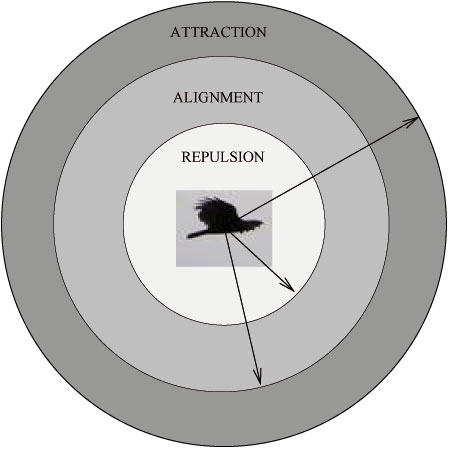
\includegraphics[height=6cm]{fig/cap03/3zones.png}}
    \caption{Modelo de las 3 zonas}
    \label{fig:3zonesModel}
\end{figure}

La zona interior es la llamada zona de repulsión o zona vital en la cual el individuo tiende a rechazar cualquier contacto con el que esté en esa zona, distanciándose. La zona de alineamiento o de orientación es en la cual tiende a igualar el mismo comportamiento que los individuos que están en esa zona. Por último, la zona de atracción o de socialización, es en la cual, los individuos que se encuentran en esa zona se acercan al individuo evitando estar lejos de los demás animales que están en esa región. Aunque el comportamiento de un grupo de animales se basa en rasgos generales en estas 3 zonas conceptuales, la realidad es que para poder reproducir un comportamiento de enjambre realista hay que incluir interacciones mucho más complicadas.

Por su parte, para demostrar que se consigue el consenso en el modelo general de Cucker Smale, los autores citados, proponen uno más general en el cual el promedio tiene en cuenta el módulo de la velocidad relativa ($ |v_{i}-v_{j}|^{p-2} $) de sus individuos (\ref{eq:CSArbor}). Obsérvese que para el valor $p = 2$ se obtiene el modelo inicial de Cucker-Smale. Mediante este modelo actualizado, demuestran que el consenso del grupo ocurre en un tiempo finito para 0 < p < 2 y 0 < $\beta$ <1/2 y con una velocidad algebraica si 2 < p < 3 - 2$\beta$ en contraste con la velocidad exponencial obtenida para el modelo estándar de Cucker-Smale con p = 2 y 0 < $\beta$ < 1/2


\begin{equation}\label{eq:CSArbor} 
    \left\lbrace
    \begin{array}{l}
        \dot{x}_{i}(t)=v_{i}(t) \\
        \dot{v}_{i}(t)= \displaystyle{\frac{1}{N}\sum_{j=1}^{N}a_{ij}(v_{j}-v_{i})|v_{i}-v_{j}|^{p-2}}
    \end{array}
    \right.
\end{equation}

Para concluir, en este artículo (\cite{canizo2010collective}) se propone un modelo en base al de atracción-repulsión (\ref{eq:attractionRepulsion}) y al general de Cucker-Smale (\ref{eq:CS5GeneralBeta}) al que llaman  ``modelo de las 3 zonas'':

\begin{equation}\label{eq:Arbor3zonesModel} 
    \left\lbrace
    \begin{array}{l}
        \dot{x}_{i}(t)=v_{i}(t) \\
        \dot{v}_{i}(t)=\displaystyle{-\frac{1}{N}\sum_{j\neq 1}\nabla U(|x_{i}-x_{j}|)+\frac{1}{N}\sum_{j=1}^{N}a_{ij}(v_{j}-v_{i})}
    \end{array}
    \begin{array}{r}
        (i = 1, ..., N) \\
        (i = 1, ..., N)
    \end{array}
    \right.
\end{equation}

En este modelo los individuos tienden a adoptar todos la misma velocidad, tal y como sucede en el modelo General de Cucker Smale, pero además consiguiendo que se agrupen todos los individuos.

\subsection{Modelo de Trelat} \label{s3_3_2}
Como se ha visto hasta ahora, el modelo de Cucker-Smale y sus diferentes mejoras, sólo llegan al consenso bajo ciertas condiciones iniciales, aunque los esfuerzos de todos los estudios se centran en obtener el modelo más óptimo para que esto ocurra. Existen muchas variaciones y extensiones del modelo de Cucker Smale, cada uno intentando resolver algunos de los problemas que puede tener ese modelo, teniendo en cuenta o añadiendo ciertos factores como aparición de ruido, fuerzas que eviten la colisión, tolerancia a errores, etc.

Para Trelat, una mayor optimización del modelo significará un menor gasto energético para que el consenso del grupo se consiga. La cita que mejor explica el razonamiento que utiliza en sus estudios es la siguiente: ``en vez de controlar a un mayor número de agentes con impulsos más pequeños, hay que actuar de manera más contundente sobre un menor número de líderes'' \cite{caponigro2015sparse}. Para entender mejor el modelo de Trelat, se debe entender antes cómo controlar el modelo de Cucker Smale. Cuando el consenso de un grupo no se ha conseguido mediante la autoorganización del grupo como puede verse en el \ref{example1} en el caso de $|arctan(x_0) + v_0| > \pi/2$ es natural
preguntarse si es posible provocar que el grupo consiga el consenso mediante una fuerza o acción externa. 

\begin{equation}\label{eq:trelat_CS}
    \left\lbrace
    \begin{array}{ll}
        \dot{x}_{i}(t)=v_{i}(t) \\
        \dot{v}_{i}(t)= \displaystyle{\frac{1}{N}\sum_{j=1}^{N} a(||x_i(t)-x_j(t)||)(v_{j}(t)-v_{i}(t))}
    \end{array}
    \right.
\end{equation}

Los autores de este estudio se refieren a este tipo de consenso con el término ``organización mediante intervención''. Para esta intervención, matemáticamente se añade al sistema propuesto por Cucker Smale \ref{eq:trelat_CS} la variable de control $u_i$. Con este término, Trelat lo que consigue es que el individuo $i$ se mueva hacia una dirección común, aportándole un empujón extra a cada individuo del grupo. 

\begin{equation}\label{eq:CSTrelat_control}
    \left\lbrace
    \begin{array}{l}
        \dot{x}_{i}(t)=v_{i}(t) \\
        \dot{v}_{i}(t)= \displaystyle{\frac{1}{N}\sum_{j=1}^{N}a(||x_{j}(t)-x_{i}(t)||)(v_{j}(t)-v_{i}(t))+u_{i}(t)}
    \end{array}
    \right.
\end{equation}

En esta ocasión, la variable de control $u_i$ se selecciona en base a la perpendicular del vector, proporcionando un ``empujón'' perpendicular al individuo en base a la siguiente ecuación. 

\begin{equation}\label{eq:Trelat_ui}
    u_i(t) = 
    \left\lbrace
    \begin{array}{l}
        \displaystyle{-\alpha_i \frac{v_{\perp_{i}}(t)}{||v_{\perp_{i}}(t)||}} \\
        0
    \end{array}
    \right.
\end{equation}

\noindent en la cual $\alpha_j$ es una constante que por simplificar, se iguala a 1, $v_{\perp_{i}}(t)$ del numerador es el vector perpendicular que va a modificar la dirección actual del individuo, y $||v_{\perp_{i}}(t)||$ en el denominador es la dirección en la que se va a proporcionar el cambio. 

Por tanto, en este estudio, lo que demuestran los autores es que en un tiempo finito el sistema consigue reunir las condiciones que Cucker y Smale dicen que asegura la convergencia a pesar de empezar en un estado que sin ningún tipo de control, el modelo inicial, no llegaría al consenso.

\chapter{Resultados simulados} \label{cap4}

\setminted[matlab]{
    xleftmargin=20pt,
    linenos,
    breaklines,
    bgcolor=gris85}

En este capítulo se ofrece una comparativa de los modelos explicados en el capítulo \ref{cap3}. Se simula mediante Matlab la evolución de un grupo de individuos que, partiendo de las mismas condiciones iniciales, se comporta de acuerdo a las reglas fijadas por cada uno de los modelos. Se proporcionan así mismo datos que corroboren los resultados.

\section{Preliminares} \label{s4_1}
Es innegable el reto matemático que supone proporcionar un modelo que replique el movimiento aparentemente aleatorio de un grupo de aves o peces, pero gracias a las herramientas informáticas que hoy en día están al alcance de nuestra mano, comprender cómo se comporta cada uno de ellos puede resultar más sencillo. El principal propósito de este capítulo, es comparar los diferentes modelos  estudiados en el capítulo anterior con una herramienta que nos permita simular el comportamiento asociado a cada modelo, aportando gráficas y datos. 

Para ello se ha utilizado Matlab, un software de programación basado en matrices, utilizado para cálculos técnicos, análisis de datos, procesamiento de señales, entre otras características que hacen que sea un programa muy utilizado en el ámbito de la ingeniería. Una de las ventajas de utilizar Matlab es que ofrece un entorno fácil de usar, optimizado para una estructura basada en matrices, como la usada en la formulación de los modelos estudiados. Es por esto que se ha optado por utilizar este software.

En las próximas secciones se proporcionarán datos y gráficas que comparen resultados que se obtienen aplicando los diferentes modelos de consenso a un grupo de individuos que partan de unas condiciones de posición y velocidad aleatorias. 

\section{Diseño} \label{s4_2}
Tanto para comparar resultados entre el mismo modelo como para hacerlo con respecto a los resultados de otros modelos, es necesario diseñar y estructurar el código de manera que sea posible configurar las condiciones iniciales y crear funciones parametrizadas que se ejecuten independientemente de estos valores iniciales.

\subsection{Condiciones iniciales}\label{s4_2_1}
Todas las comparativas y pruebas que se han hecho en este capítulo y que se explicarán a lo largo de éste, parten de unas mismas condiciones iniciales. 
Las condiciones iniciales de las que parten todas las comparativas y pruebas que se exponen a lo largo de este capítulo son la utilización de 20 individuos, que se mueven en una ventana temporal de 20 a 60 segundos con incrementos de 0.1 segundos.

\begin{listing}[!ht]
\begin{minted}{matlab}
    n=20;
    h=0.1;
    Tmax=20; 
    t=0;
\end{minted}
\caption{Parámetros de la simulación}
\end{listing}

Para que las pruebas tengan sentido, todos los modelos parten de una repartición aleatoria de los elementos. Para ello se generan una matriz aleatoria de 20x4 con números de 0 a 1 en la cuales, las columnas 1 y 2 se reservan para definir las posiciones de cada uno de los elementos y las columnas 3 y 4 para generar números entre -2 y 4 que definirán el vector velocidad de cada uno de los elementos de la siguiente manera:

\begin{listing}[!ht]
\begin{minted}{matlab}
    XVi=rand(n,4);
    XVi(:,[3:4])=XVi(:,[3:4])*6-2;
\end{minted}
\caption{Generación de posiciones y velocidades aleatorias}
\end{listing}

Para comprender mejor la manera en la que se genera la posición y velocidad inicial de manera aleatoria para cada uno de los elementos veamos el caso del primer elemento (primera fila de la matriz):

\begin{enumerate}
    \item Se generan los números aleatorios. Ver tabla \ref{tab:XVi1}
    \item Las dos primera columnas definen la posición.
    \item Para tener números aleatorios entre -2 y 4, se multiplican por 6 y se dividen por 2 las dos últimas columnas. Ver tabla \ref{tab:XVi2}.
    \item Las dos primera columnas definen la posición y las dos últimas definen el vector posición. Ver imagen \ref{fig:posInicial}.
\end{enumerate}

\begin{table}[!h]
\caption{Generación de números aleatorios}
    \begin{center}
        \begin{tabular}{| c | c | c | c |}
            \hline
            $x$ & $y$ & $u$ & $v$ \\
            \hline
            0.8147 & 0.6557 & 0.4387 & 0.7513 \\
            \hline
            ... & ... & ... & ... \\
            \hline
        \end{tabular}
        \label{tab:XVi1}
    \end{center}
\end{table}
\begin{table}[!h]
\caption{Generación de los componentes $x$ e $y$ del vector velocidad}
    \begin{center}
        \begin{tabular}{| c | c | c | c |}
            \hline
            $x$ & $y$ & $u$ & $v$ \\
            \hline
            0.8147 & 0.6557 & \textbf{0.6325} & \textbf{2.5076} \\
            \hline
            ... & ... & ... & ... \\
            \hline
        \end{tabular}
        \label{tab:XVi2}
    \end{center}
\end{table}

\begin{figure}[!h]
  \centering
    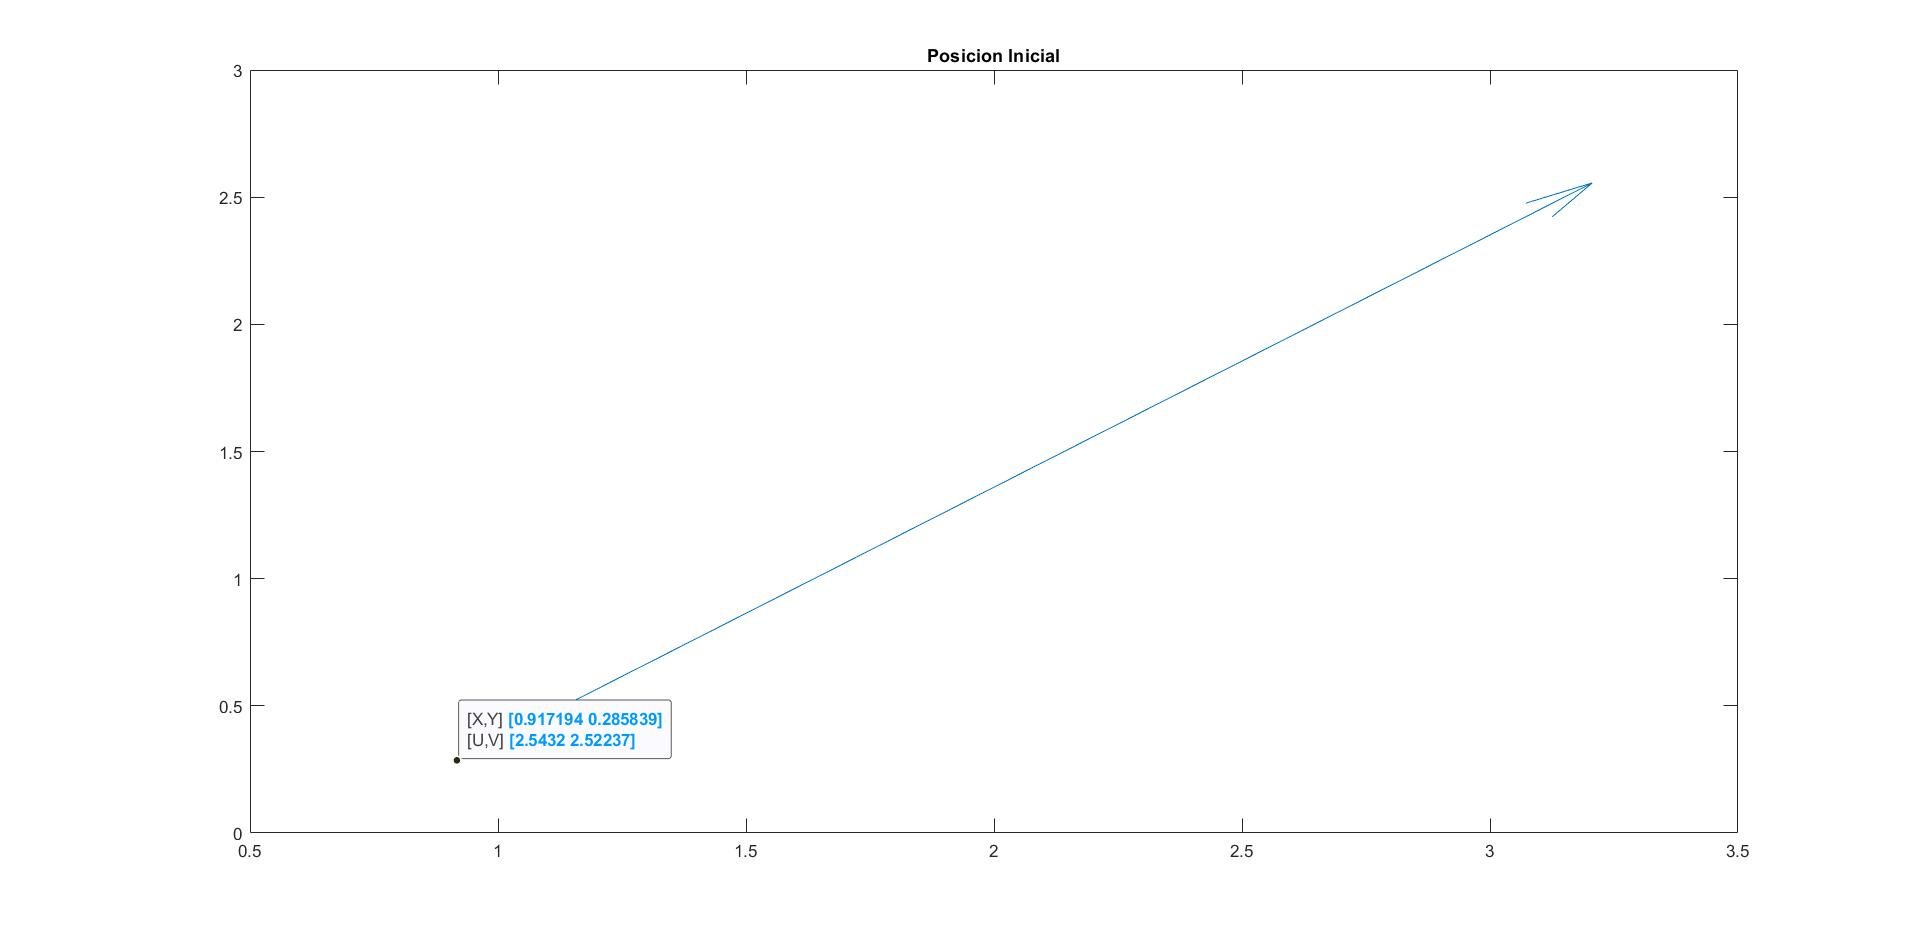
\includegraphics[scale=0.2]{fig/cap04/unelemento.jpg}
  \caption{Posición y velocidad inicial de un agente}
  \label{fig:posInicial}
\end{figure}


El comportamiento de este vector velocidad será el objeto de nuestro estudio en las próximas secciones. 
\subsection{Aplicación de los modelos}\label{s4_2_2}
En cada iteración pasa lo siguiente:
\begin{itemize}
    \item Se provee a cada modelo de una matriz de 20x4 con las posiciones y velocidades de todos los elementos (ver código fuente \ref{src:comparativa} 1-37).
    \item A esos datos se les aplica el modelo de consenso correspondiente. Las funcionen desarrolladas pueden verse en los anexos \ref{src:cs0}, \ref{src:csarbor}, \ref{src:cstrelat1}, \ref{src:cstrelat2}
    \item El modelo devuelve otra matriz 20x4 con los datos modificados (\ref{src:comparativa} 34-37, 50-53)
    \item Se guarda en una lista las diferencias de velocidades en cada iteración en cada modelo. (\ref{src:comparativa} 61, \ref{src:maxdif})
    \item Se representan las nuevas posiciones y velocidades de los 20 individuos en las n gráficas diferentes de los modelos a comparar(\ref{src:comparativa} 64-95)
\end{itemize}

\subsection{Comparativa y gráficas de simulación de comportamiento}\label{s4_2_3}
Durante toda la ejecución, se observa en una gráfica cómo se modifica en cada iteración el movimiento de cada elemento. 
Una vez finalizada la ejecución, se representan en otra gráfica cómo han cambiado los vectores velocidad a lo largo del tiempo en cada modelo gracias a la lista que se ha ido guardando de la media de las diferencias del vector velocidad. 

\begin{figure}[h]
  \centering
    \includesvg[scale=0.2]{fig/cap04/elementos.svg}
  \caption{Comportamiento de cada modelo}
\end{figure}

\subsection{Diferencia máxima de velocidad}\label{s4_2_4}
Aunque visualmente en las pruebas se puede ver cómo los vectores poco a poco tienden a una dirección común, notar esto en cada iteración es complicado y por ello se va a ir obteniendo una gráfica de la diferencia máxima que existe en un momento dado con respecto a la media del grupo según la ecuación \ref{eq:vmax}.

\begin{equation}\label{eq:vmax}
    \begin{array}{l}
        v_{max} = \displaystyle{\max\left(\|v_{i}-\frac{1}{N}\sum_{j=0}^{N}\vec{v_{j}}\|\right)}
    \end{array}
    \begin{array}{r}
        (i= 0, ..., N)
    \end{array}
\end{equation}

En las gráficas que representan la evolución de este dato a lo largo de la ejecución el eje de ordenadas es relativo a la máxima diferencia de todo el grupo y el eje de abscisas representa el tiempo en milisegundos.

\section{Modelo general de Cucker Smale} \label{s4_3}
Antes de mostrar gráficamente cómo afecta la aplicación de un modelo de control a Cucker-Smale y de comparar los diferentes controles propuestos por los autores vistos en el capítulo anterior, es necesario comprender cómo el modelo general de Cucker-Smale afecta al vector velocidad de cada uno de los individuos que conforman un grupo de animales, ya sea una bandada de pájaros, un banco de peces o cualquier animal social de los vistos con anterioridad. 

Las pruebas sobre este modelo se hacen en función del parámetro $\beta$ que como ya se ha comentado, la condición indispensable para que se llegue al consenso, es que tenga un valor $\beta \leq 1/2$. A continuación mostramos dos casos generales con dos valores de $\beta$ diferentes.

\subsection{Caso 1: se llega al consenso} \label{s4_3_1}
Para demostrar cómo aplicando el modelo de Cucker-Smale se llega al consenso, se elige una $\beta = 0.25$. 

\begin{figure}[htbp]
\centering
    \subcaptionbox{Posición inicial\label{fig:pos-i}}{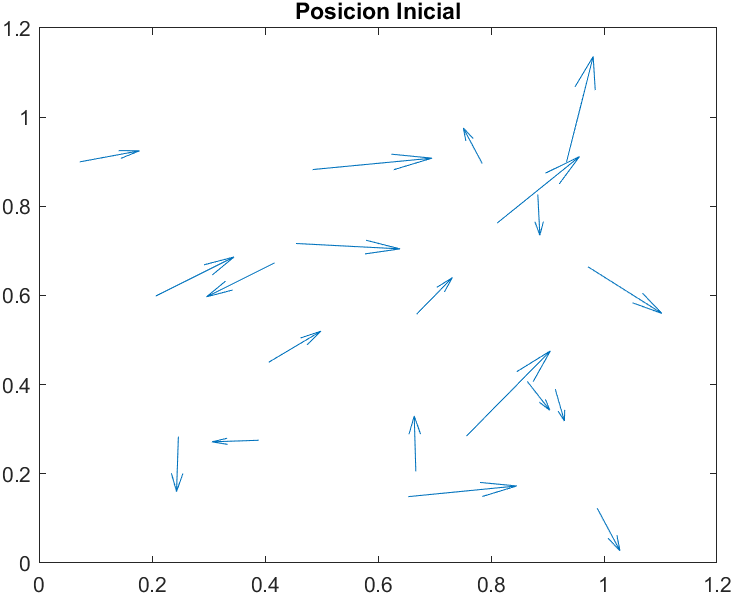
\includegraphics[height=5.5cm]{fig/cap04/1CSB025/posicion_inicial.png}}
    \subcaptionbox{Posición final\label{fig:pos-f}}{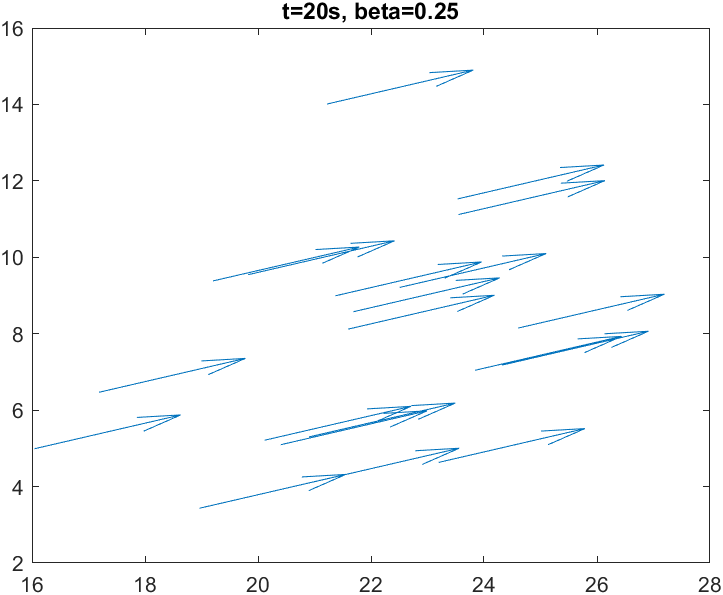
\includegraphics[height=5.5cm]{fig/cap04/1CSB025/posicion_final.png}}
\caption{Evolución del grupo en un tiempo t=20s} 
\label{fig:CS025_pos}
\end{figure}

Esta simulación se ha hecho utilizando un tiempo de 20s y se puede observar en las figuras (fig. \ref{fig:CS025_pos}) como partiendo de una posición y velocidades totalmente aleatorias en el espacio, todos los vectores han terminado convergiendo hacia el mismo. En la figura \ref{fig:CS025_vel} obtenemos una gráfica en la que se ve cómo con el paso del tiempo, la diferencia entre el vector más alejado es menor con respecto a la media de los demás. 
\begin{figure}
    \centering
    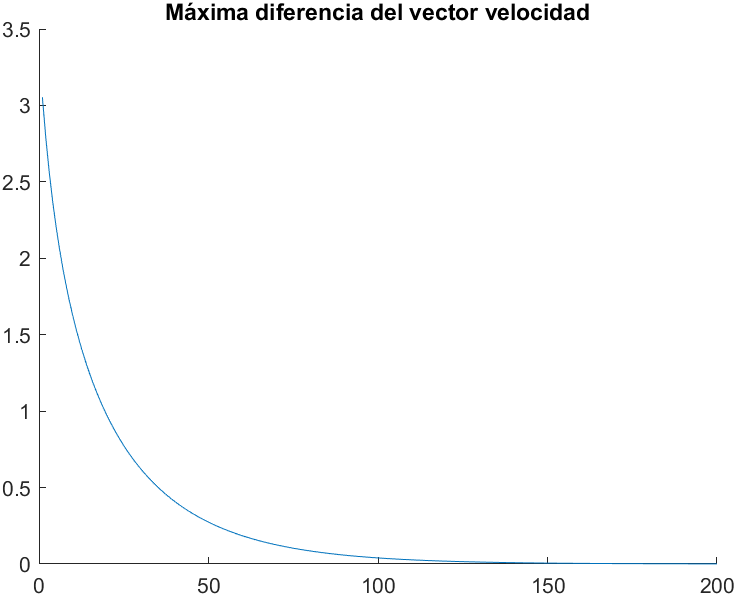
\includegraphics[height=5.5cm]{fig/cap04/1CSB025/velocidad.png}
    \caption{Evolución de la diferencia de velocidades}
    \label{fig:CS025_vel}
\end{figure}

Según los datos, en el segundo 20 la máxima diferencia de la velocidad de un elemento con respecto a la media sigue existiendo ($\|\vec{v_i}\|-\|\Bar{v}\| \approx 0.0010$) y para poder disminuir este valor se han hecho otras simulaciones aumentando el tiempo de ejecución, llegando  a obtener una diferencia $\|\vec{v_i}\|-\|\Bar{v}\| \approx 3.1451\cdot10^{-8}$ en un tiempo de simulación de $t=60s$. Esto muestra que esta diferencia tiende a 0 y además el ratio de decaimiento es significativo con una configuración del parámetro de convergencia $\beta\leq0.5$, tal y como dicen Cucker y Smale en su estudio. 

\subsection{Caso 2: se produce la dispersión} \label{s4_3_2}
Para demostrar cómo aplicando el modelo de Cucker-Smale el grupo se dispersa, se elige un valor del parámetro $\beta = 0.75$ obteniendo con cualquiera de las simulaciones, un resultado final similar al que se muestra en la figura \ref{fig:CS075_pos}.

\begin{figure}[htbp]
\centering
    \subcaptionbox{Posición inicial\label{fig:pos-i-075}}{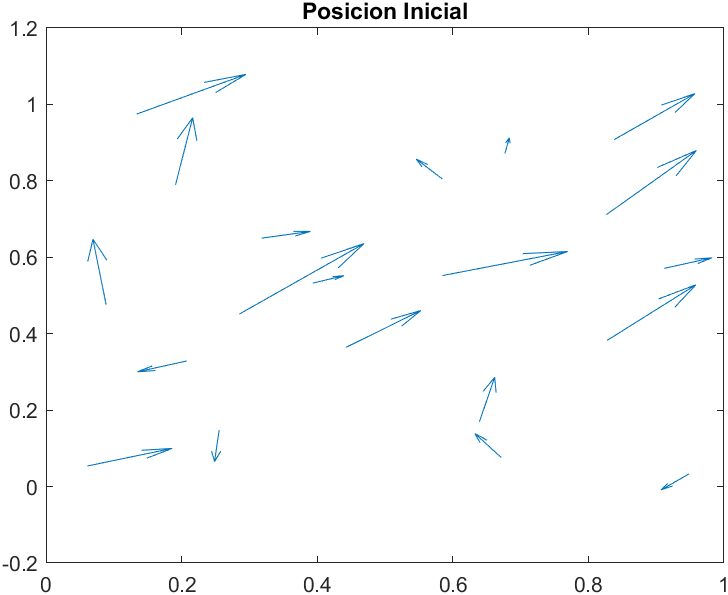
\includegraphics[height=5.5cm]{fig/cap04/2CSB075/posicion_inicial.png}}
    \subcaptionbox{Posición final\label{fig:pos-f-075}}{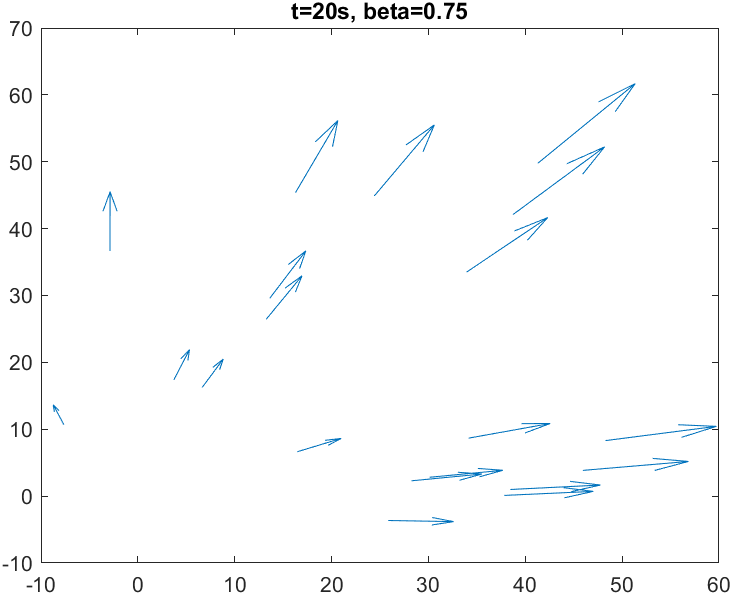
\includegraphics[height=5.5cm]{fig/cap04/2CSB075/posicion_final.png}}
\caption{Evolución del grupo en un tiempo t=20s} 
\label{fig:CS075_pos}
\end{figure}

Se han realizado adicionalmente varias ejecuciones, cada una con diferentes tiempos de simulación, para asegurarse de que los vectores de velocidad nunca llegan al consenso tendiendo a un valor que nunca es 0 para diferentes tiempos finitos (ver fig. \ref{fig:CS075_vel}) aunque no se puede determinar si las curvas tienden a un valor positivo o a cero, a un ritmo cada cada vez más lento en el tiempo, lo que es compatible con el teorema de Cucker Smale que dice que con una $\beta>0.5$ siempre se puede producir el consenso del grupo en un tiempo infinito, si se dan las condiciones iniciales adecuadas.

\begin{figure}[htbp]
\centering
    \subcaptionbox{t=20}{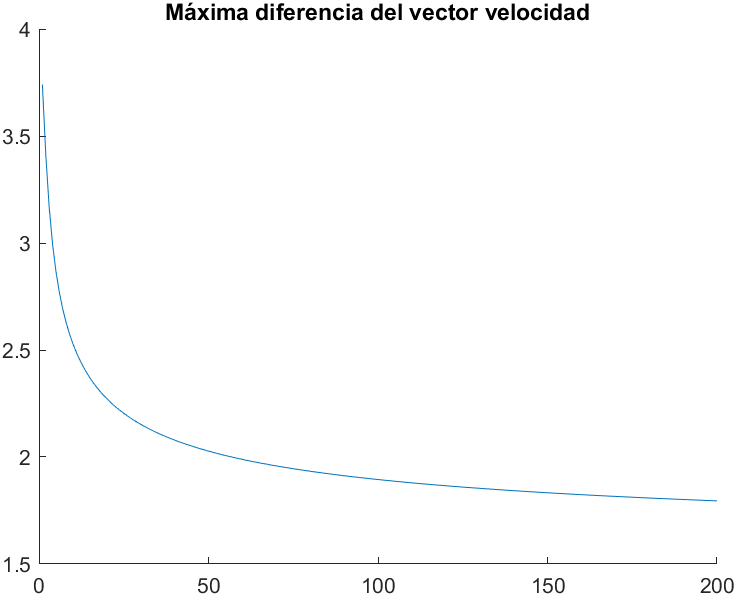
\includegraphics[height=5.5cm]{fig/cap04/2CSB075/velocidad20s.png}}
    \subcaptionbox{t=60(1)}{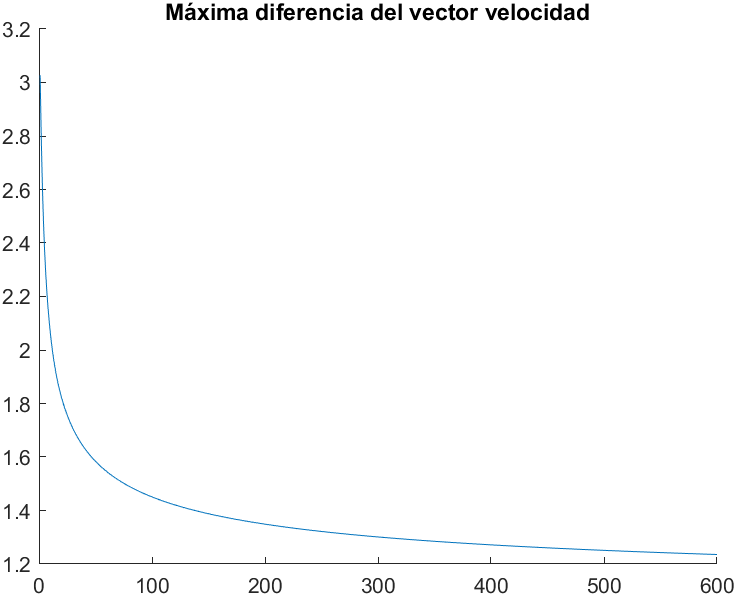
\includegraphics[height=5.5cm]{fig/cap04/2CSB075/velocidad60s1.png}}
    \subcaptionbox{t=60(2)}{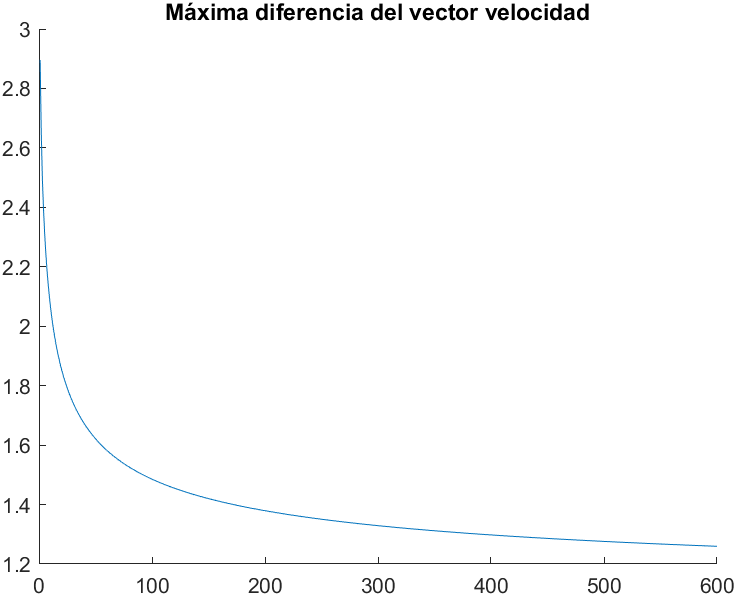
\includegraphics[height=5.5cm]{fig/cap04/2CSB075/velocidad60s2.png}}
    \subcaptionbox{t=120}{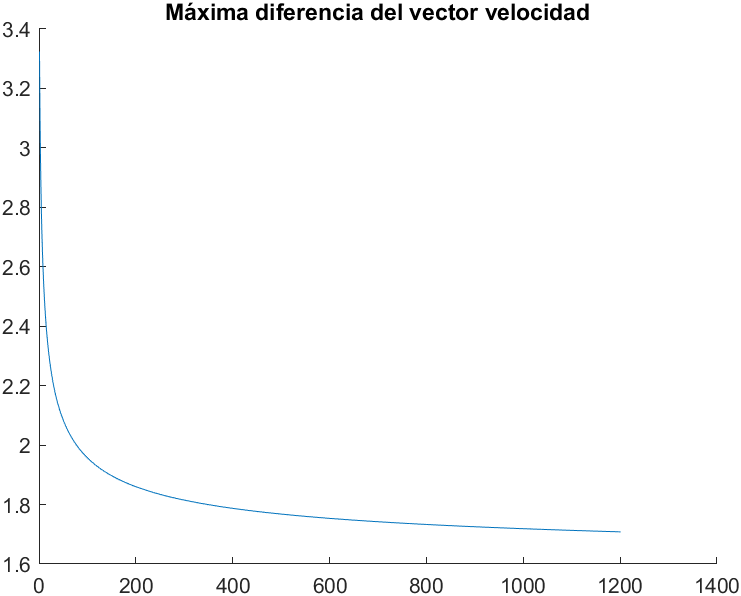
\includegraphics[height=5.5cm]{fig/cap04/2CSB075/velocidad120s.png}}
\caption{Evolución de la diferencia de velocidades con $\beta=0.75$} 
\label{fig:CS075_vel}
\end{figure}

Otra simulación que se ha hecho es minimizar la diferencia de los vectores velocidad de todos los miembros para generar una condición bajo la cual se llegue al consenso con un \linebreak $\beta > 0.75$ (figura \ref{fig:CS075_consenso}) pudiéndose observar y analizar desde dos puntos de vista. Por una parte, en la figura \ref{fig:CS075_consenso} se muestra que cuando la diferencia de estos vectores es suficientemente pequeña ($\pm 30^o$ en la dirección de los vectores), se llega al consenso. 

Por otra parte, teniendo en cuenta la figura \ref{fig:CS075_comparacion_consenso} también se puede observar cómo a medida que aumenta la diferencia inicial de estos vectores, el estado de consenso tarda más en producirse, hasta llegar a un punto en el que la diferencia es demasiado grande como para que se pueda producir la alineación del vector velocidad en un tiempo finito en el que pueda realizarse la simulación.

\begin{figure}[htbp]
\centering
    \subcaptionbox{Posición inicial}{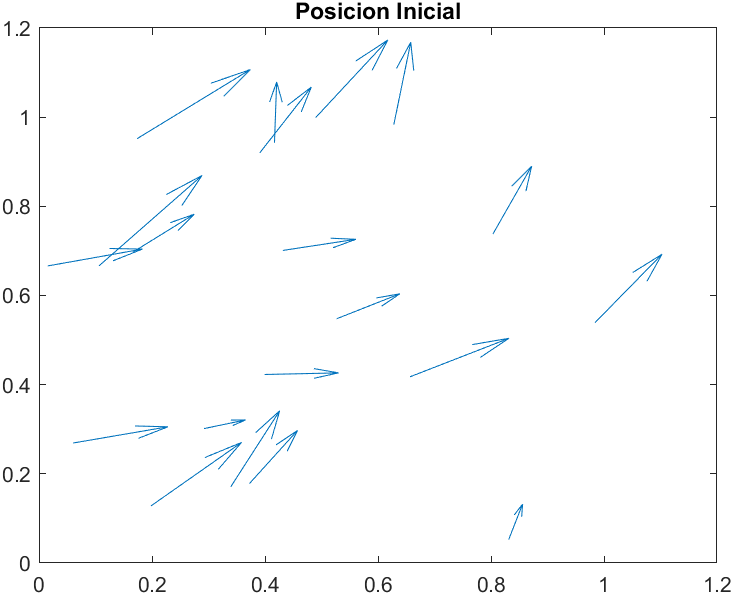
\includegraphics[height=5.5cm]{fig/cap04/2CSB075/consenso/posicion0102.png}}
    \subcaptionbox{Posición final}{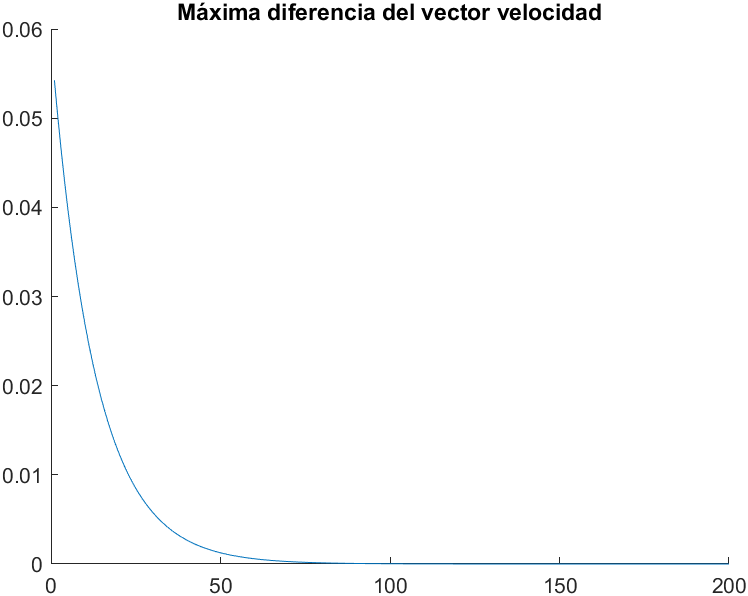
\includegraphics[height=5.5cm]{fig/cap04/2CSB075/consenso/velocidad0102.png}}
\caption{Consenso con una $\beta > 0.5$} 
\label{fig:CS075_consenso}
\end{figure}

\begin{figure}[!ht]
    \centering
    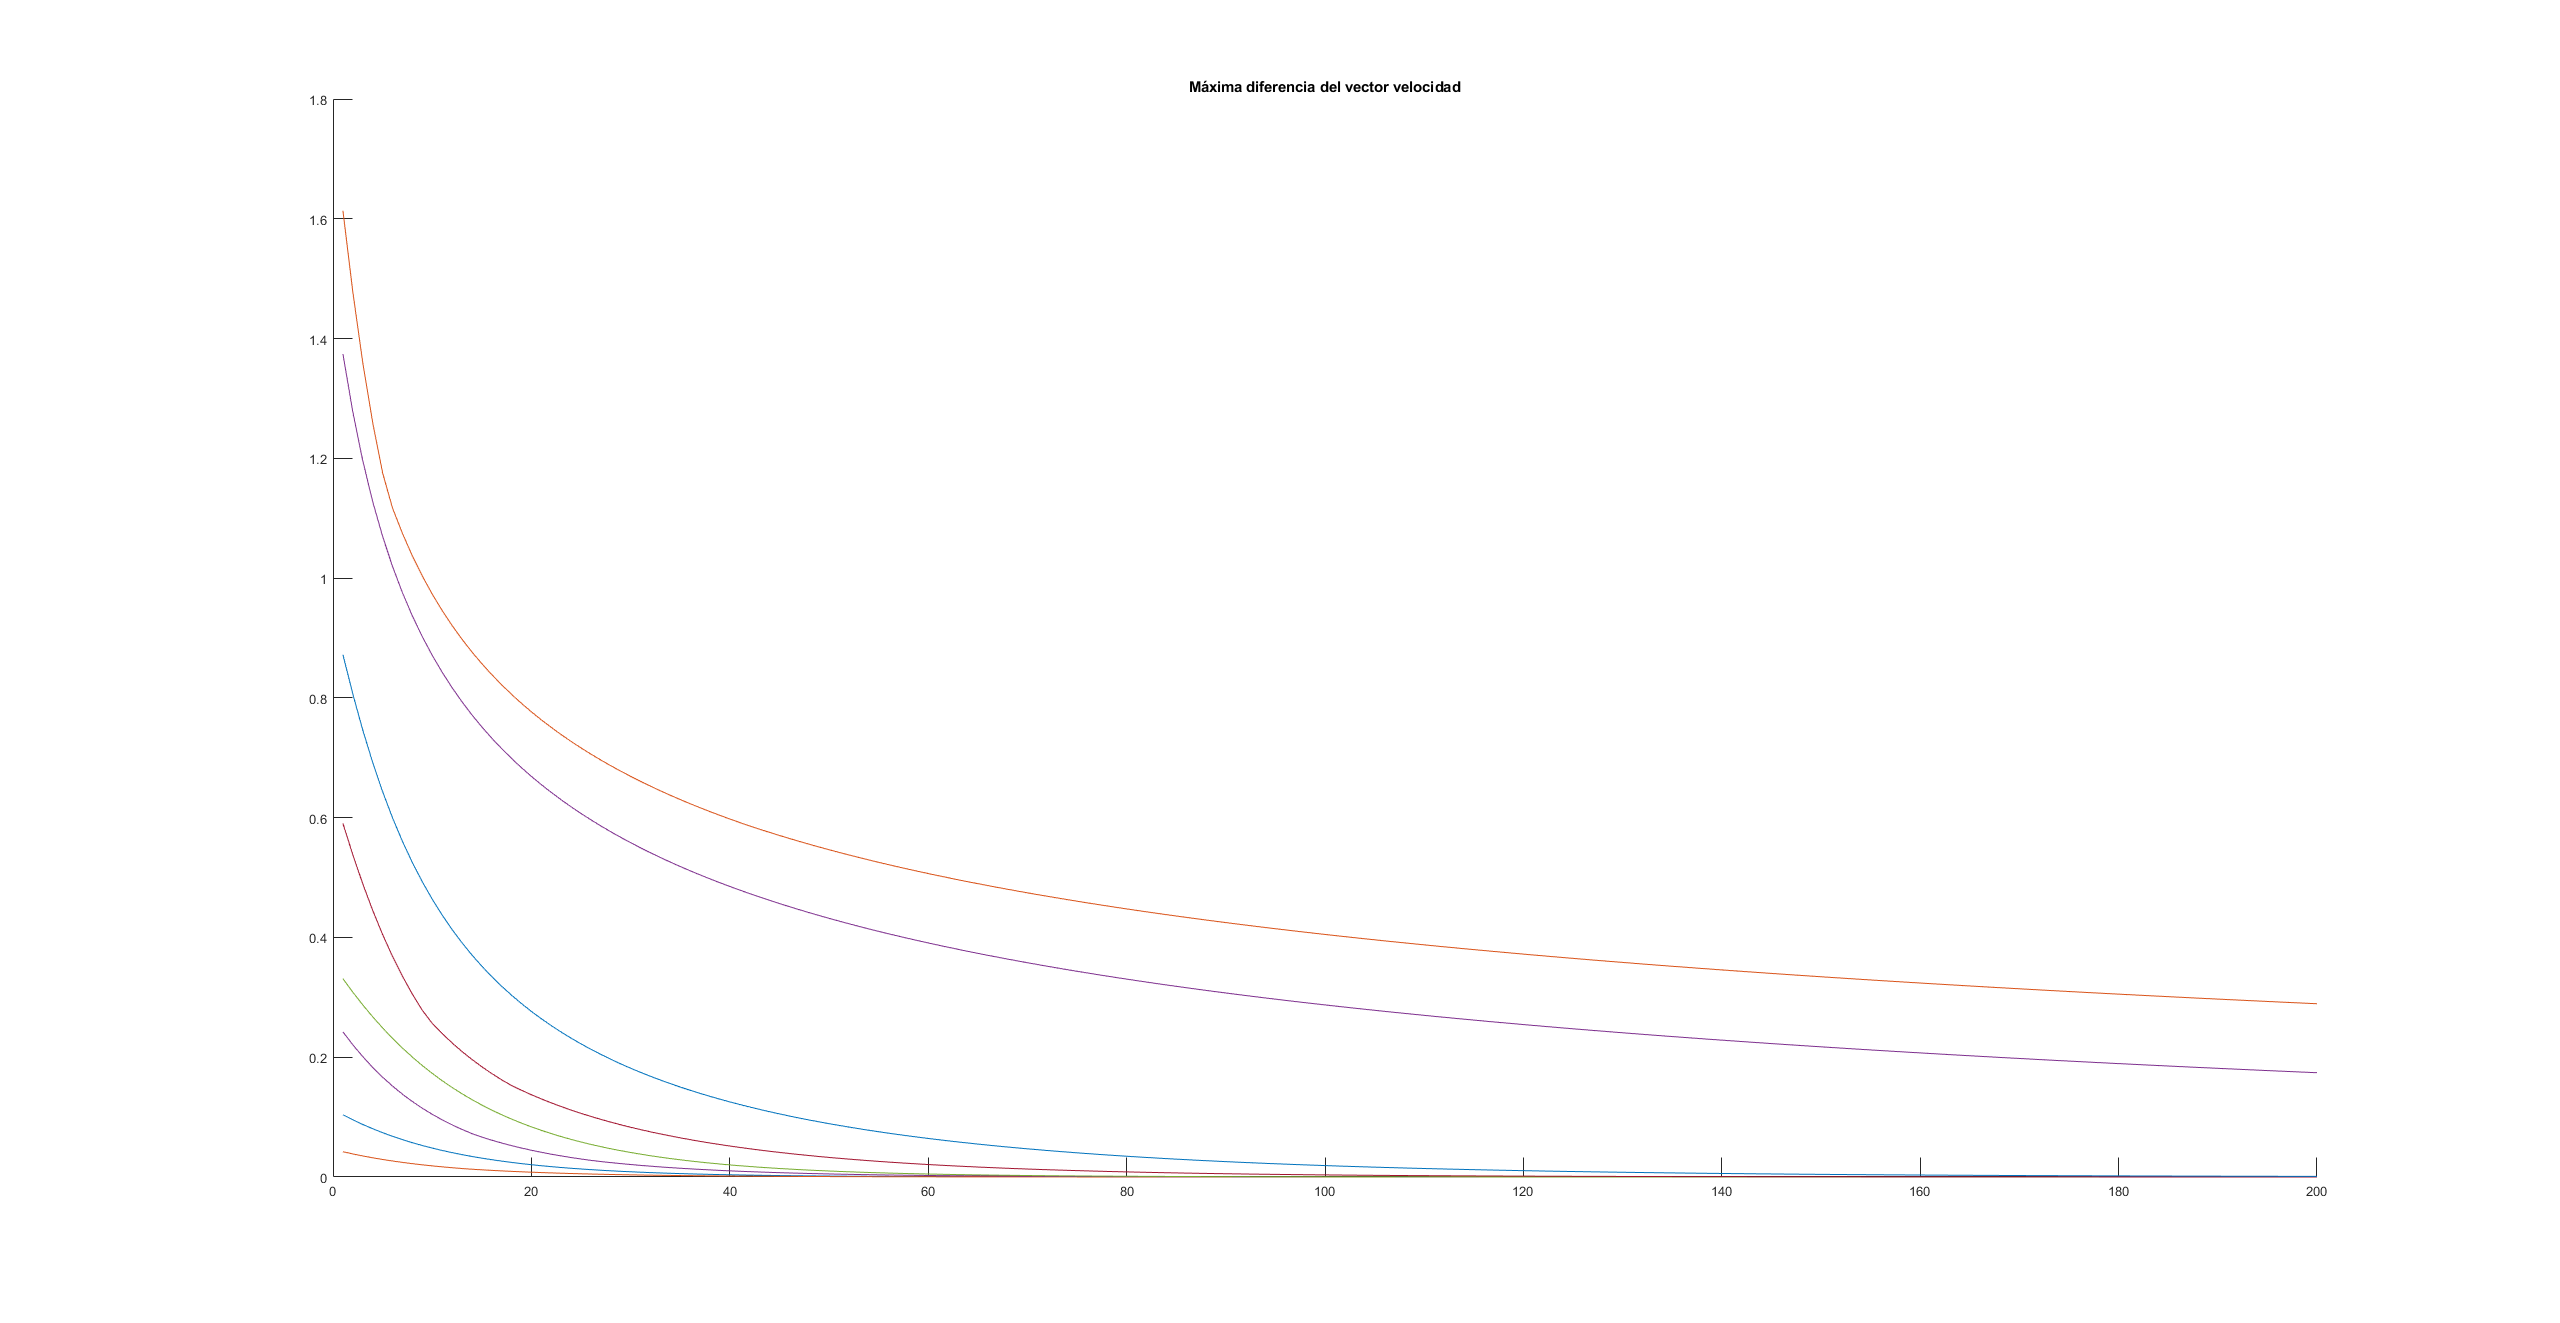
\includegraphics[width=\textwidth]{fig/cap04/2CSB075/consenso/todas.png}
    \caption{Comparación del comportamiento con respecto a la diferencia inicial cuando $\beta > 0.5$}
    \label{fig:CS075_comparacion_consenso}
\end{figure}

%\newpage
%\clearpage

\section{Aplicación de controles al modelo general de Cucker-Smale} \label{s4_4}

Una vez analizado y probado el modelo de Cucker Smale de manera práctica, se añaden a ese modelo los controles que se han visto en el capítulo anterior. Por una parte, se añade el control de CCR añadiendo su simulación a la gráfica y por otra parte se añaden dos controles diferentes basados en el modelo de Trelat, para poder comparar también cuál es la diferencia entre controlar todos los elementos a la vez dando un pequeño empujón a todos y modificar de forma más agresiva el más alejado, proporcionando el empujón únicamente a ese vector. 

En todo este capítulo se entiende que el grupo ha llegado al consenso cuando la diferencia máxima de velocidad sea inferior o igual a $0.01$.

\subsection{Comparación entre modelos en una ejecución}
En una primera ejecución aislada, se pretende comparar los 4 modelos diferentes y el comportamiento de los elementos $N=20$ durante un tiempo finito $t=20s$ con un valor de $\beta$ que facilite el consenso en todos los casos, $\beta=0.25$.

Tal y como se ha comentado en la sección \ref{s4_2_1}, se parte de una posición y dirección aleatoria de todos los elementos pero igual entre los 4 modelos tal y como se muestra en la figura \ref{fig:pos_inicial_4models}.

\begin{figure}[!h]
    \centering
    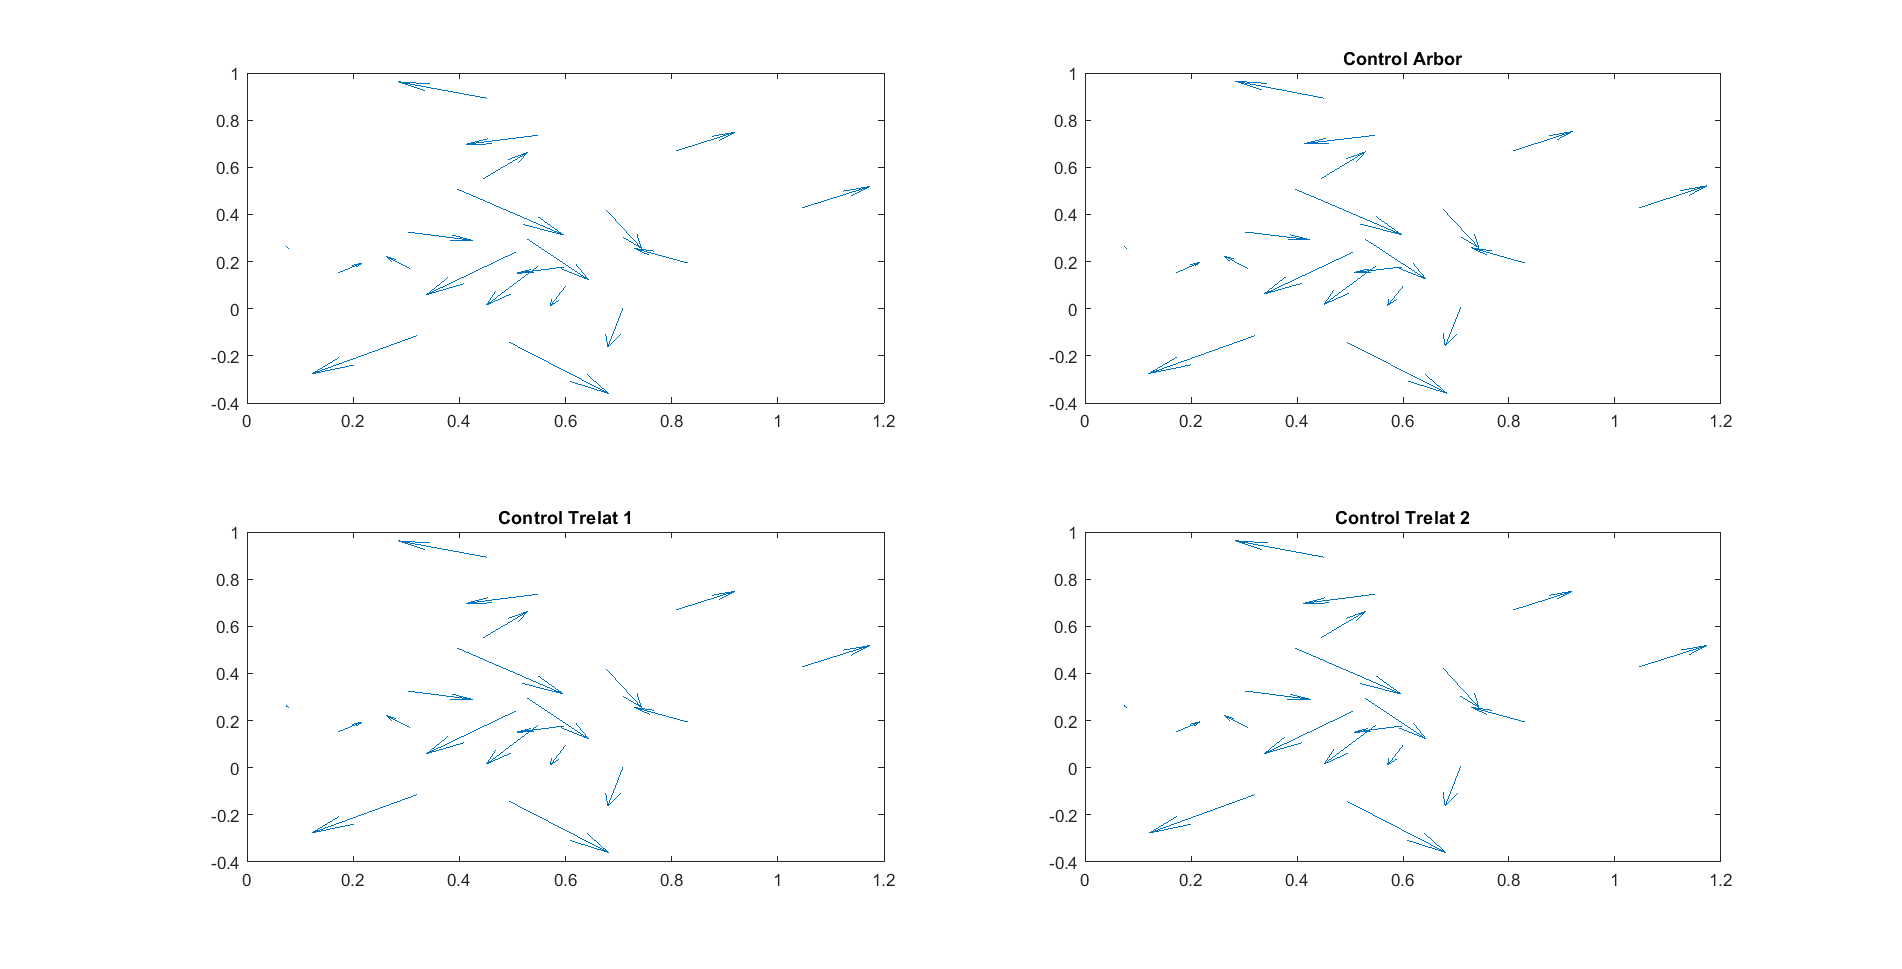
\includegraphics[width=\textwidth]{fig/cap04/3ALLB025/pos_inicial.png}
    \caption{Posición inicial de los 4 modelos.}
    \label{fig:pos_inicial_4models}
\end{figure}

Pasados los 20 segundos de ejecución, el estado de los individuo termina siendo el que se muestra en la figura \ref{fig:pos_final_4models} pudiendo observarse que los 4 modelos han conseguido llegar a una dirección común con la configuración inicial explicada.

\begin{figure}[h!]
    \centering
    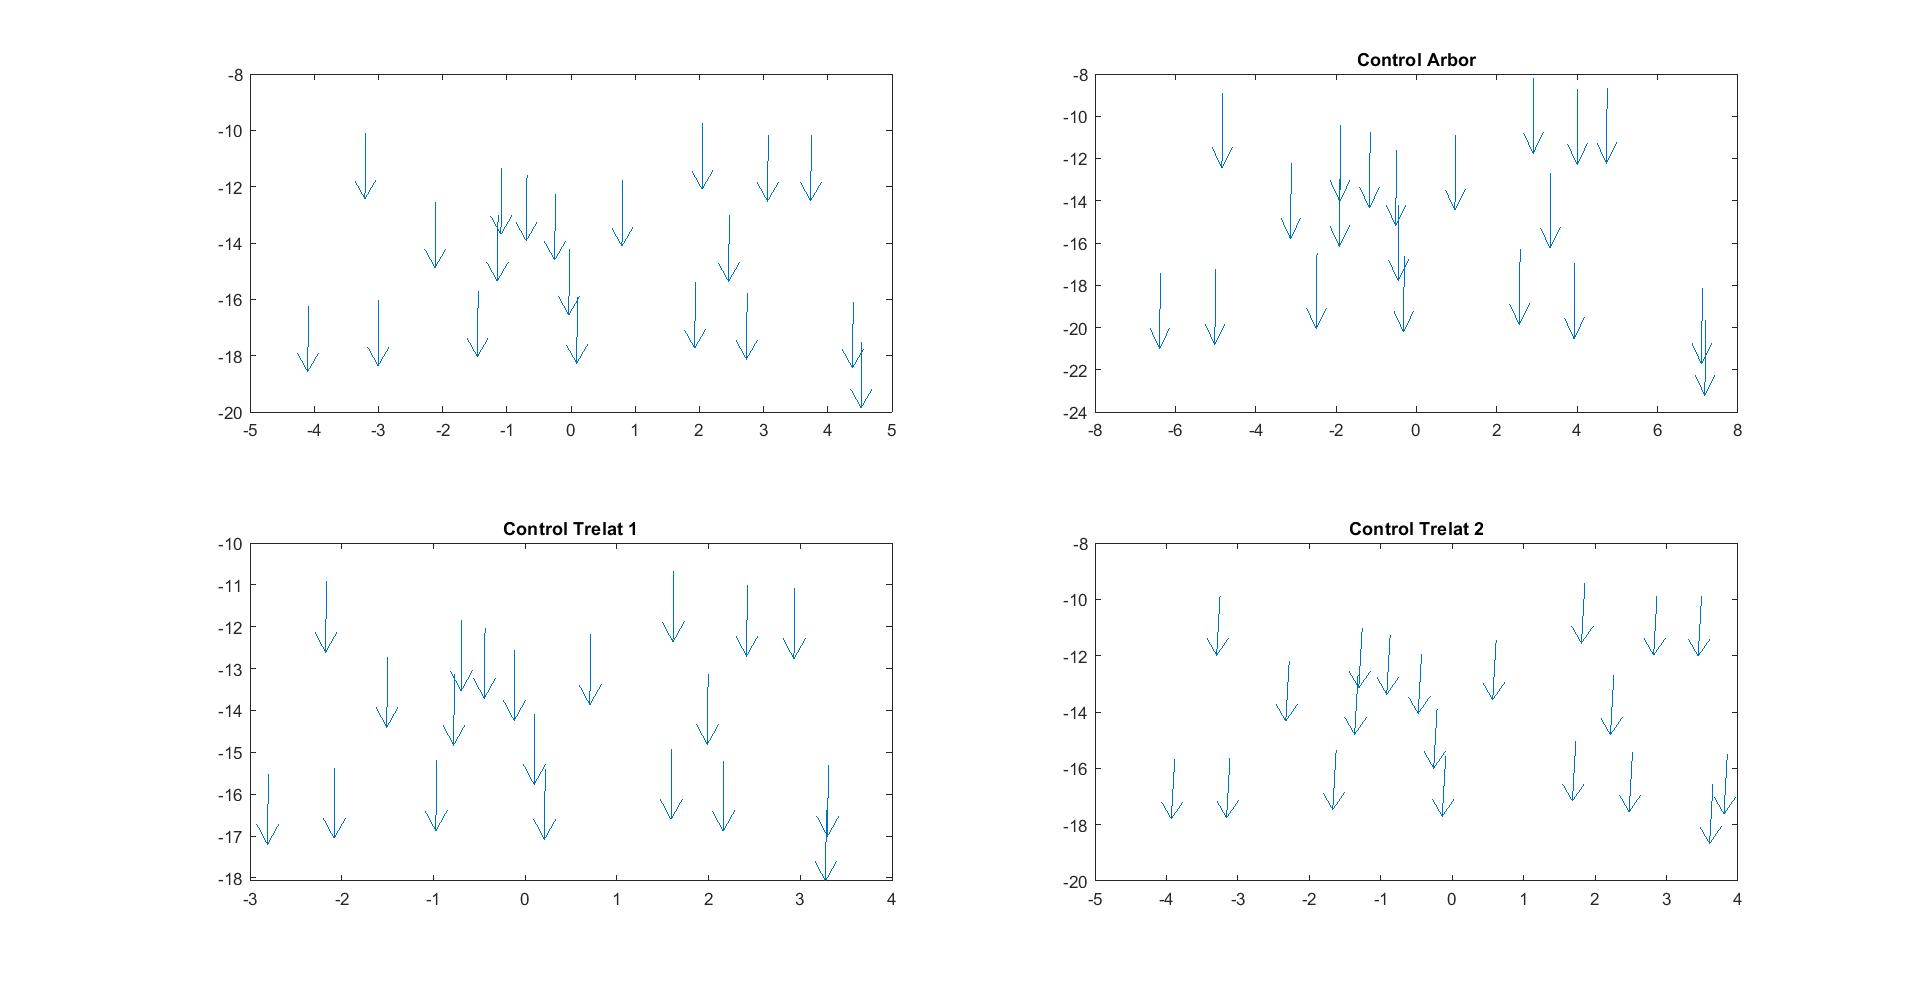
\includegraphics[width=\textwidth]{fig/cap04/3ALLB025/pos_final.png}
    \caption{Posición final de consenso de los 4 modelos.}
    \label{fig:pos_final_4models}
\end{figure}

Para poder hacer un estudio más exhaustivo del comportamiento en el tiempo de los 4 casos, en cada iteración se ha almacenado la máxima diferencia que hay entre todos los vectores en cada uno de los casos tal y como se ha explicado en la sección \ref{s4_2_4} de este mismo capítulo. 

Con estos datos se pretende obtener una gráfica que pueda comparar a qué velocidad se llega al consenso.

\begin{figure}[htbp]
\centering
    \subcaptionbox{Velocidad de consenso}{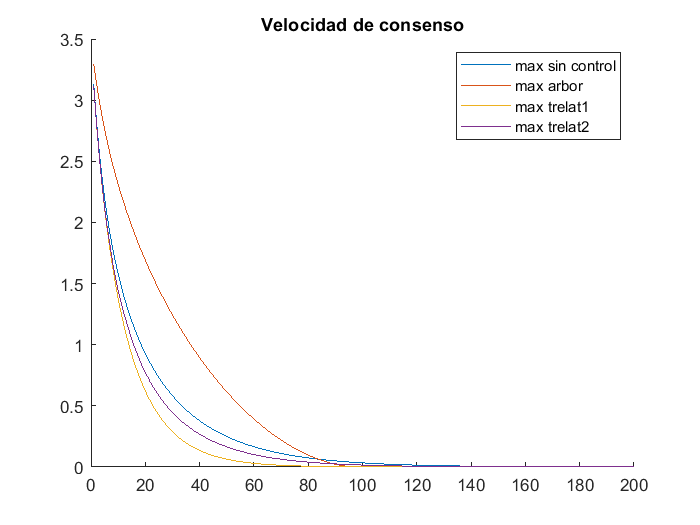
\includegraphics[height=5cm]{fig/cap04/3ALLB025/vel_consenso.png}}
    \subcaptionbox{Velocidad de consenso final ampliada}{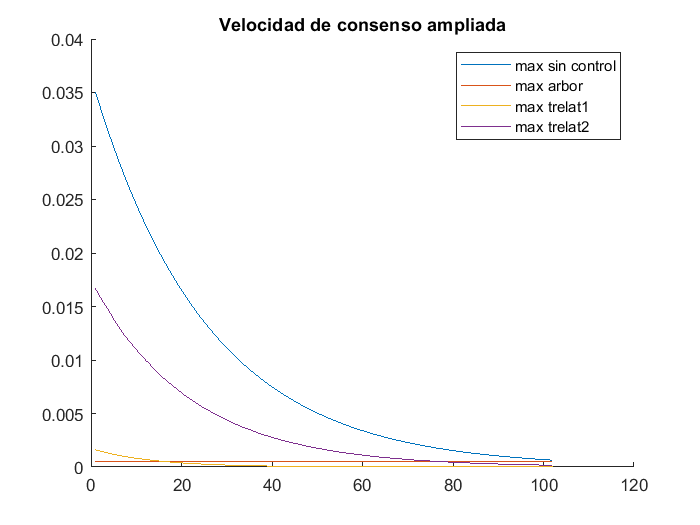
\includegraphics[height=5cm]{fig/cap04/3ALLB025/vel_consenso_ampliada.png}}
\caption{Comparación de la velocidad a la que se adquiere el consenso con $\beta = 0.25$.} 
\label{fig:consenso_4models}
\end{figure}

Un primer vistazo a la figura \ref{fig:consenso_4models}(a) sirve para corroborar que los 4 modelos terminan llegando al consenso en el tiempo fijado, con la diferencia de que cada uno lo hace a una velocidad diferente. Si se amplia la gráfica a los momentos finales donde parece que todos los modelos llegan al consenso (figura \ref{fig:consenso_4models}(b)) se puede analizar mejor qué ha sucedido en cada caso pudiendo así sacar varias conclusiones:

\begin{enumerate}
    \item El modelo de Cucker Smale sin ningún tipo de control añadido, es el último en llegar al consenso.
    \item El control que se propone en CCR, es el que tiene menos pendiente en la velocidad de consenso y el que antes llega (se puede ver en la gráfica ampliada que cuando Cucker Smale, y los dos de Trelat están todavía disminuyendo su máxima diferencia, el modelo de CCR ya ha llegado al consenso. 
    \item Entre los dos de Trelat, ambos llegan al consenso aunque Trelat2, que tiene menos gasto energético a la hora de controlar el modelo de CS, tarda más en obtener el estado de consenso.
\end{enumerate}

Se corrobora pues, gracias a estas simulaciones, que bajo las mismas condiciones iniciales y con una $\beta = 0.25$ todos los modelos llegan al consenso para un tiempo finito $t=20s$ habiendo una clara mejora cuando se aplica algún tipo de control sobre el modelo de Cucker Smale.

Si concluimos esta prueba configurando una $\beta=0.75$ y $t=120s$ entonces obtenemos que en el tiempo finito establecido los dos modelos que son capaces de obtener el consenso son los dos de Trèlat según la gráfica de la figura \ref{fig:consenso_4models_b075} mientras que Cucker Smale y CCR no lo han logrado en ese tiempo, aunque sí que lo harían si pudiera simularse un tiempo infinito.

\begin{figure}[htbp]
\centering
    \subcaptionbox{Velocidad de consenso}{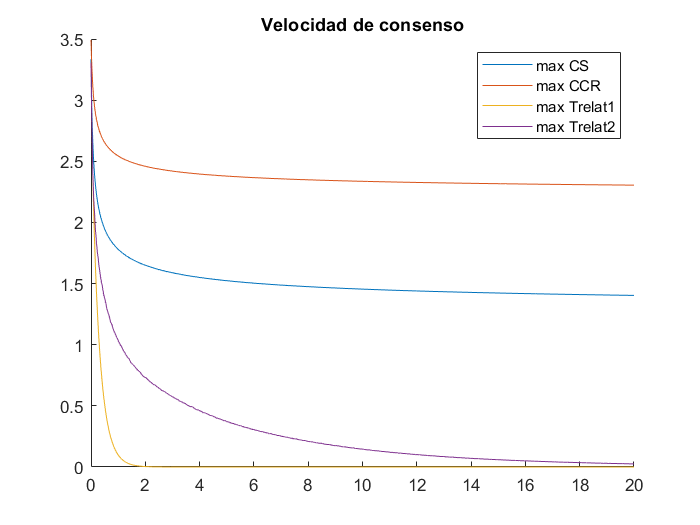
\includegraphics[height=5cm]{fig/cap04/4ALLB075/velocidad.png}}
    \subcaptionbox{Velocidad de consenso final ampliada}{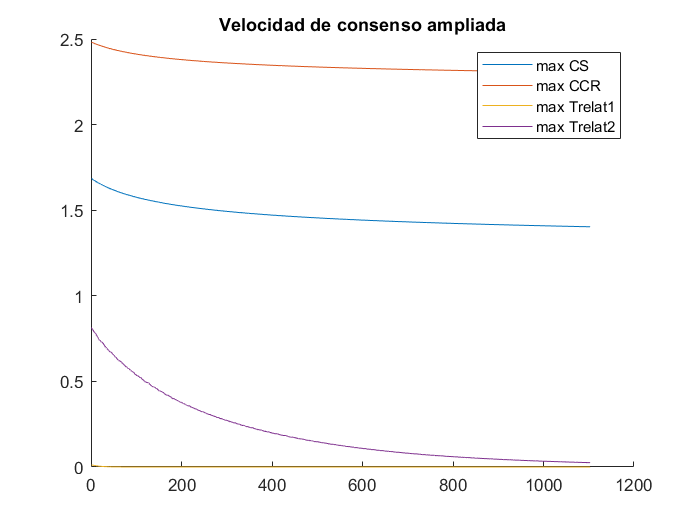
\includegraphics[height=5cm]{fig/cap04/4ALLB075/velocidad_ampliada.png}}
\caption{Comparación de la velocidad a la que se adquiere el consenso con $\beta=0.75$.} 
\label{fig:consenso_4models_b075}
\end{figure}

\subsection{Comparación entre ejecuciones}

Para descartar que los resultados obtenidos anteriormente sean objeto del azar y de una configuración específica del estado inicial del grupo, es necesario repetir esas pruebas una cantidad suficiente de veces cambiando las condiciones iniciales para obtener una media de datos que corroboren lo anterior.

Para ello se ha decidido comparar el momento en el que se llega al consenso partiendo de 500 posiciones iniciales diferentes. Es necesario aclarar en este punto, que al igual que en la sección anterior, se ha tomado la decisión de definir el momento en el que se considera que el grupo ha llegado al consenso, cuando la diferencia del módulo del vector más alejado con respecto a la media de la dirección del grupo, es igual o menor que $0.01$, es decir, $||v_{max}||$.

\begin{table}[!ht]
\caption{Tiempos de consenso en 500 ejecuciones con $\beta=0.25$ y $t=20s$}
    \centering
    \begin{tabular}{|l|l|l|l|l|}
    \hline
        \textbf{Nº Ejecución} & \textbf{$T_c$ CS} & \textbf{$T_c$ CCR} & \textbf{$T_c$ Trelat 1} & \textbf{$T_c$ Trelat 2} \\ \hline
        1 & 14 & 10,1 & 7,5 & 11,9 \\ \hline
        2 & 13,8 & 9,7 & 7,6 & 10,9 \\ \hline
        3 & 14,6 & 10 & 7,6 & 11,7 \\ \hline
        4 & 13,3 & 9,2 & 7,4 & 11,4 \\ \hline
        5 & 15,6 & 12,2 & 7,9 & 12,9 \\ \hline
        6 & 14,6 & 11 & 7,7 & 12,2 \\ \hline
        7 & 15,3 & 11 & 7,8 & 11,6 \\ \hline
        8 & 15,5 & 11,9 & 7,9 & 12 \\ \hline
        9 & 13,2 & 9 & 7,4 & 10,9 \\ \hline
        10 & 13,3 & 9 & 7,4 & 10,9 \\ \hline \hline
        ... & ... & ... & ... & ...\\ \hline \hline
        497 & 13,9 & 9,6 & 7,5 & 11,2 \\ \hline
        498 & 15,5 & 11,5 & 7,8 & 12,7 \\ \hline
        499 & 14,9 & 11,2 & 7,7 & 12,7 \\ \hline
        500 & 15,2 & 11,7 & 7,8 & 11,4 \\ \hline \hline
        \textbf{Promedio} & \textbf{14,4586} & \textbf{10,8066} & \textbf{7,6586} & \textbf{11,7518} \\ \hline
    \end{tabular}
    \label{tab:tiemposConsenso}
\end{table}

En la tabla \ref{tab:tiemposConsenso} se han cortado algunos resultados pero se puede observar claramente cuál es el modelo más efectivo para llegar antes al consenso, siendo el de Trèlat que impulsa en en cada iteración a todos sus elementos. Esto resulta coherente ya que este modelo impulsa a todos los elementos a la vez.

Se ha repetido el proceso anterior, llevando a cabo  500 repeticiones de la simulación, fijando el valor del parámetro $\beta$ en  $\beta=0.5$. En este caso ha sido necesario ampliar el tiempo de ejecución a $t=60s$. En este caso es curioso observar cómo por un lado el modelo de Cucker Smale sin aplicarle ningún control sólo consigue el consenso del grupo en 2 ocasiones mientras que el primer modelo de Trélat si que lo consigue en todas las ejecuciones. En la tabla \ref{tab:tiemposConsensoB05} se muestran algunos de los resultados obtenidos en esta prueba, entre los que se encuentran los más característicos:

\begin{table}[!h]
\caption{Tiempos de consenso en 500 ejecuciones con $\beta=0.5$ y $t=60s$}
    \centering
    \begin{tabular}{|l|l|l|l|l|}
    \hline
        \textbf{Nº Ejecución} & \textbf{$T_c$ CS} & \textbf{$T_c$ CCR} & \textbf{$T_c$ Trelat 1} & \textbf{$T_c$ Trelat 2} \\ \hline
        5 & 60 & 60 & \cellcolor{green!15}9,6 & \cellcolor{green!15}44,2 \\ \hline
        6 & 60 & 60 & \cellcolor{green!15}9,9 & 60 \\ \hline \hline
        11 & 60 & 60 & \cellcolor{green!15}9,5 & \cellcolor{green!15}41,8 \\ \hline
        12 & \cellcolor{green!15}51,8 & \cellcolor{green!15}38,1 & \cellcolor{green!15}8,4 & \cellcolor{green!15}23,4 \\ \hline \hline
        58 & 60 & 60 & \cellcolor{green!15}9,6 & \cellcolor{green!15}50,3 \\ \hline
        59 & 60 & 60 & \cellcolor{green!15}9,8 & 60 \\ \hline \hline
        139 & 60 & 60 & \cellcolor{green!15}9,5 & \cellcolor{green!15}39,3 \\ \hline
        140 & 60 & 60 & \cellcolor{green!15}9,5 & 60 \\ \hline \hline
        216 & 60 & 60 & \cellcolor{green!15}9,6 & \cellcolor{green!15}50,3 \\ \hline
        217 & 60 & 60 & \cellcolor{green!15}9,5 & 60 \\ \hline \hline
        243 & 60 & 60 & \cellcolor{green!15}9,3 & \cellcolor{green!15}36,2 \\ \hline
        244 & 60 & 60 & \cellcolor{green!15}9,9 & 60 \\ \hline \hline
        290 & 60 & 60 & \cellcolor{green!15}9,3 & \cellcolor{green!15}38,6 \\ \hline
        291 & 60 & 60 & \cellcolor{green!15}9,6 & 60 \\ \hline \hline
        388 & 60 & 60 & \cellcolor{green!15}9,2 & \cellcolor{green!15}42,1 \\ \hline
        389 & 60 & 60 & \cellcolor{green!15}9,8 & 60 \\ \hline \hline
        440 & 60 & 60 & \cellcolor{green!15}8,9 & \cellcolor{green!15}28,8 \\ \hline
        441 & 60 & \cellcolor{green!15}55,2 & \cellcolor{green!15}8,6 & \cellcolor{green!15}31,2 \\ \hline \hline
        477 & 60 & 60 & \cellcolor{green!15}9,3 & \cellcolor{green!15}44,9 \\ \hline
        478 & \cellcolor{green!15}57,2 & \cellcolor{green!15}53,5 & \cellcolor{green!15}8,5 & \cellcolor{green!15}26,5 \\ \hline \hline
        499 & 60 & 60 & \cellcolor{green!15}9,3 & \cellcolor{green!15}50,6 \\ \hline
        500 & 60 & 60 & \cellcolor{green!15}8,8 & \cellcolor{green!15}41,3 \\ \hline \hline
        \textbf{Total} & \textbf{2} & \textbf{3} & \textbf{500} & \textbf{493} \\ \hline
    \end{tabular}
    \label{tab:tiemposConsensoB05}
\end{table}

Analizando los datos de la tabla puede observarse que en el caso de $\beta=0.5$, aunque los modelos de Cucker Smale y CCR solo hayan llegado al consenso en 2 y 3 ocasiones respectivamente, el segundo de ellos, consigue una menor dispersión de sus elementos.

Por último, se ha hecho una prueba con una $\beta=0.75$ y cambiando un poco código se ha pretendido realizar una ejecución eliminando el límite del tiempo de la ejecución, y simplemente definiendo el final de la ejecución cuando lo 4 modelos hayan llegado al estado que hemos definido de consenso. El resultado ha sido que los dos modelos de Trélat han conseguido el estado de consenso en un tiempo de 10s y 141s respectivamente, frente a los otros dos modelos que en un tiempo de 60 días no han logrado disminuir suficientemente la diferencia entre los vectores de dirección de sus elementos como para llegar al estado de consenso. Esto no quiere decir que no puedan llegar nunca, pues estos valores siguen disminuyendo a lo largo del tiempo a pesar de hacerlo de manera muy lenta.
\chapter{Conclusiones y trabajos futuros} \label{ch:conclusiones}

\section{Conclusiones} \label{s5_1}
Estudiar patrones que se dan de forma natural en el entorno que nos rodea puede resultar un reto debido a la aparente aleatoriedad en todo lo que sucede pero a la vez que complejo, resulta interesante cuando se valora la opción de poder aplicar estos comportamientos de la naturaleza y de otros seres vivos en soluciones de nuestro día a día.

Gracias a una lectura exhaustiva de los estudios y trabajos más importantes que se han basado en estos patrones, se ha adquirido una visión general de qué comportamientos existen en el medio natural y de qué manera pueden ser útiles para nosotros. Tal y como se pretendía, como primeros objetivos (O1 y O2) cumplido se ha aprendido cómo y para qué se organizan algunos insectos tan conocidos como las hormigas o las abejas, o animales como los peces o las aves, distinguiendo dos maneras de organización colectiva, una atendiendo a los elementos individuales y otra con una visión mucho más general relativa al grupo en su conjunto. 

Como objeto principal de este trabajo tenemos conocer en profundidad el modelo de Cucker Smale y dos modelos adicionales que lo controlan, el modelo propuesto por Cañizo et al. \cite{canizo2010collective} y el propuesto por Trèlat et al. \cite{caponigro2015sparse}. En el capítulo \ref{cap3} se han entendido cada uno de ellos desde el aspecto teórico, conociendo pues, que Cucker Smale basa su modelo en el comportamiento colectivo de las aves, aportando un sistema de ecuaciones que responde y es capaz de simular ese comportamiento en función, principalmente, del llamado parámetro de convergencia, $\beta$. Es en un función de este parámetro, que una bandada de pájaros simulada, conseguiría o no llegar al consenso siendo para $\beta\leq0.5$ siempre apto para conseguirlo en un tiempo finito y para $\beta>0.5$ solamente apto para llegar al consenso en tiempo finito bajo una condición de posición y direcciones concretas aunque siempre podría hacerlo en un tiempo infinito (objetivo O3). Por otra parte, en CCR, los autores proponen un modelo de Cucker Smale al cual añaden la influencia que ejercen unos individuos sobre otros en función del promedio de la velocidad relativa del grupo demostrando que a parte de las condiciones del parámetro de consenso $\beta$ de Cucker Smale, con este modelo también se consigue el consenso y la agrupación de todos los individuos para $0<p<2$. El modelo de control de Trèlat, basa sus estudios en una premisa muy clara que es el gasto energético que conlleva controlar el grupo para conseguir el consenso, centrándose así en generar un impulso mayor de manera individual sobre individuo más desviado, en vez de hacerlo sobre todo el grupo a la vez. Para ello compara cada uno con la media de las velocidades del grupo. Con esto, puede darse como completado el objetivo O4.

Todos los modelos anteriores se han probado en Matlab de manera que fuera posible obtener datos sobre los que apoyar los resultados obtenidos. Por una parte se ha comparado el comportamiento del modelo de Cucker Smale en función del parámetro $\beta$ realizando ejecuciones con valores que favorezcan el consenso en un tiempo finito ($\beta=0.25$) así como con valores que no lo hagan ($\beta=0.75$) obteniendo que en el primer caso el grupo es capaz de llegar al consenso en un tiempo $t<20s$, al contrario que en el segundo caso (objetivo O6)

En el caso de las pruebas realizadas para contrastar el comportamiento del modelo de Cucker Smale, con los que le controlan (objetivo O5), se ha podido comprobar la efectividad de los diferentes controles, que permiten llegar al consenso de manera más rápida. Se han comparado para ellos 4 modelos diferentes: Cucker Smale, CCR, Trèlat impulsando a todos los individuos y Trèlat impulsando sólo al que presenta mayor diferencia con la media del grupo (objetivo 7 y 8) llegando a dos conclusiones principales, por una parte que el modelo de CCR es el más rápido en llegar a un estado de consenso y el de Trèlat que impulsa sólo a un individuo consigue llegar al consenso con menor gasto energético, en un tiempo finito ligeramente mayor. 

Por último se han hecho pruebas masivas en las que se pudiera comprobar que el consenso no depende de la posición inicial de una ejecución, si no que se cumple independientemente de la posición y dirección iniciales del grupo, simulando los 4 modelos con 500 estados iniciales diferentes, obteniendo que lo que se ha explicado en el párrafo anterior se cumple en la mayoría de los casos.


\section{Trabajos futuros} \label{s5_2}
Como se ha podido ver en el presente trabajo, los estudios relacionados con \textit{swarming} y el comportamiento colectivo tiene gran importancia, habiendo conseguido grandes avances en las últimas décadas. No obstante, seguir investigando y explorando nuevos modelos en la actualidad puede resultar de gran utilidad de cara a poder utilizarlos en aplicaciones cada vez más avanzadas. Se proponen varias lineas de trabajo futuros que según lo estudiado sin de gran interés:
\begin{itemize}
    \item En línea con trabajo actual, se propone añadir a las pruebas ya realizadas, el concepto de consenso del grupo propuesto por Cucker y Smale en el teorema 2 de su artículo \cite{cucker2007mathematics}, en vez del estado de consenso que se ha tomado en este trabajo como una diferencia máxima del vector velocidad menor que $0.01$. 
    \item También relacionado con este TFG, sería de gran interés realizar más pruebas utilizando el límite del parámetro de convergencia, $\beta = 0.5$ probando con diferentes estados iniciales de posición y velocidad, comparando el comportamiento con los otros modelos.
    \item Ejercer controles más avanzados en los que se añaden conceptos como el sorteo de obstáculos fijos y obstáculos móviles. Esto puede aplicarse para dotar a cada individuo de cierta inteligencia en cuanto a la detección de sus propios compañeros \cite{alejo2014optimal, berg2011reciprocal, van2008reciprocal}
    \item La clara relación con el mundo de la robótica y de los vehículos aéreos no tripulados (drones) permite pensar en una línea de investigación muy interesante con una gran cantidad de aplicaciones relacionadas con el control y la gestión aérea de problemas cotidianos. 
    
\end{itemize}


% Los anexos pueden ir en la misma carpeta que el cuerpo del documento 
% porque eso facilita la migración de partes de un capítulo a un anexo.
\appendix\cleardoublepage
\hypertarget{ch:anexos}{%
    \chapter{Código de Matlab} \label{a1}

\section{Funciones} \label{a1_functions}
Para poder realizar todas las simulaciones se han generado distintas funciones bajo la premisa de que puedan ser reutilizables para poder alimentarlas con una serie de parámetros referentes a la posición y dirección de cada elemento en un momento dado, y que cada una de las funciones ejerza el control del modelo al que hace referencia en cada caso.

\subsection{Cucker Smale}\label{a1_1_CS}

\lstinputlisting[language=Matlab,
    caption=Función que simula comportamiento de Cucker Smale,
    label=src:cs0
]{tex/source_code/cs0.m}

\subsection{CCR}\label{a1_2_CCR}
\lstinputlisting[language=Matlab,
    caption=Función que simula comportamiento según CCR,
    label=src:cs_arbor
]{tex/source_code/cs_arbor.m}

\subsection{Trèlat 1}\label{a1_3_trelat1}
\lstinputlisting[language=Matlab,
    caption=Función que simula comportamiento de Trélat impulsando todos los individuos,
    label=src:cs_trelat1
]{tex/source_code/cs_trelat1.m}

\subsection{Trèlat 2}\label{a1_4_trelat2}
\lstinputlisting[language=Matlab,
    caption=Función que simula comportamiento de Trélat impulsando un individuo,
    label=src:cs_trelat2
]{tex/source_code/cs_trelat2.m}

\subsection{Obtener máxima diferencia de los vectores}\label{a1_5_max_dif}
\lstinputlisting[language=Matlab,
    caption=Función que extrae el vector más alejado de cada modelo,
    label=src:max_dif
]{tex/source_code/dibujar_max_dif.m}

\section{Scripts} \label{a2_scripts}
\subsection{Comparativa de los 4 modelos}\label{a2_1}
\lstinputlisting[language=Matlab,
    caption=Script que compara el el comportamiento de las diferentes funciones,
    label=src:comparativa
]{tex/source_code/comparativa.m}

\subsection{Repetición masiva de pruebas}\label{a2_2}
\lstinputlisting[language=Matlab,
    caption=Script que repite 500 veces cada comparación,
    label=src:comparativa_500
]{tex/source_code/comparativa_noh_tc.m}


}

% La bibliografía no suele ir numerada porque se pone después de los anexos.
% No se debe poner antes de los anexos porque si se cita una referencia en
% un anexo sería una backward reference, que deben evitarse a toda costa
\cleardoublepage
\hypertarget{ch:bibliografia}{%
    \printbibliography[heading=bibintoc]}
\cleardoublepage

\end{document}
